\documentclass{biophys-new}
\usepackage[utf8]{inputenc}
\usepackage{graphicx}
\usepackage[colorlinks,allcolors=cyan!70!black]{hyperref}
\usepackage{enumitem}

\usepackage{lipsum}

\title{Model of cochlear microphonic offers insight into the tuning and magnitude of hair cell transduction current}
\author[1,*]{Brian Frost}
\author[2,3]{Elizabeth S. Olson}
\affil[1]{Electrical Engineering, Columbia University, New York, New York}
\affil[2]{Otolaryngology, Head and Neck Surgery, Columbia University, New York, New York}
\affil[3]{Biomedical Engineering, Columbia University, New York, New York}

\runningtitle{Cochlear microphonic predicts hair cell responses}

\runningauthor{Brian Frost and Elizabeth S. Olson}

\corrauthor[*]{eao2004@columbia.edu, b.frost@columbia.edu}

\papertype{Article}


\begin{document}

\begin{frontmatter}

\begin{abstract}
The mammalian cochlea relies on the active forcing of sensory outer hair cells (OHCs) to amplify traveling wave responses along the basilar membrane (BM). These forces are the result of electromotility, wherein current through the OHCs leads to conformational changes in the cells that provide stresses on surrounding structures. OHC transducer current can be detected via the voltage in the scala tympani (the cochlear microphonic, CM) and the CM can be used as an indicator of healthy cochlear operation. The CM represents a summation of OHC currents (the inner hair cell contribution is known to be small) and to use CM to probe the properties of OHC transduction requires a model that simulates that summation.  We developed a finite element model for that purpose. The pattern of current generators (the model input) was initially based on BM displacement, with the current size based on \textit{in vitro} data. The model was able to reproduce the amplitude of experimental CM results reasonably well when the input tuning was enhanced slightly (peak increased by $\sim$6 dB), which can be regarded as additional hair bundle tuning, and with a current/input value of 200-260 pA/nm, which is $\sim$4 times greater than the largest \textit{in vitro} measures. 
\end{abstract}

\begin{sigstatement}
Hair cells within the cochlea generate a current when their stereocilia pivot. A vector sum of these currents, known as the cochlear microphonic, can be measured in scala tympani. We developed a finite element model for the electrical properties of the cochlea, which we use to study the generation of the cochlear microphonic, and thereby stereocilia motion. We provide an interpretation of locality of the cochlear microphonic in terms of relative conductances within the cochlea. We find that relative to transverse basilar membrane motion, the stereocilia motion that results in hair cell current must be slightly more highly tuned. We also provide an estimate of channel sensitivity \textit{in vivo} that is larger than what has been measured \textit{in vitro}.
\end{sigstatement}
\end{frontmatter}
\clearpage
\section{Introduction}
\par{Sensory hair cells produce an electrical current due to the pivoting motion of their stereocilia hair bundle (HB). This current leads to intracellular voltage changes that drive transmitter release in the case of inner hair cells (IHC) and drive electromotility and cochlear amplification in the case of outer hair cells (OHCs) \cite{olson2020}.  The  transducer current passes through the hair cell membranes into scala tympani (ST) and produces a time-varying voltage, referred to as the cochlear microphonic (CM). Both IHCs and OHCs produce a transducer current, but the current produced by OHCs is the dominant contributor to the CM  \cite{dallos2}. The relationship between ST voltage and OHC current is complicated, as it depends on the currents of many OHCs stimulated at different amplitudes and phases according to the traveling wave response of the cochlea. The measured voltage will depend on the location where it is measured within the ST, as nearby OHCs contribute more to the locally measured voltage than those that are far away. Near the BM, voltage responses resemble local BM traveling wave responses, creating what is referred to as the \textit{local} cochlear microphonic (LCM). The LCM has been used as an indirect measure of local OHC current, and used to probe the operation of the cochlear amplifier \cite{dongolson,wang,charaziak,fridberger}.  }

\par{To use LCM data most productively, one would like to relate it more concretely to HB motion.  That project confronts, and speaks to, two unknown relationships. The first is the relationship between BM motion, which is known in the base for many species, and HB stimulation. HB pivoting has been approximated as directly proportional to BM motion \cite{dallos3}. However, the HBs are stimulated by motions within the OC, and optical coherence tomography (OCT) based measurements of motions within the organ of Corti (OC) have found that intra-OC motion can be substantially larger than BM motion \cite{renpnas2016,cooper,fallah,strimbu,chen_2011}.  Moreover, in mice HB motion has been inferred to be more sharply tuned around the peak frequency than BM motion \textcolor{blue}{via measurements of tectorial membrane (TM) and reticular lamina (RL) motions} \cite{lee}. The second unknown relationship is that between OHC current and ST voltage. Here we present a semi-cylindrical FEM of the gerbil cochlea ST which incorporates the three spatial dimensions of the fluid space and the electrical properties of the outer wall (Fig. \ref{geometry}). With this relatively physically realistic model for current spread, we compare predicted and measured CM. We are primarily concerned with two questions, and the information revealed by their answers: 1) Is the \textit{shape} of the experimentally measured LCM voltage consistent with proportionality between BM displacement and OHC current?  This question is motivated in part by an intuitive surprise at how sharply tuned the experimental LCM is \cite{dongolson,fridberger,fallah,wang}, given that it is due to a summation of distributed currents. 2) Is the \textit{magnitude} of the experimentally measured LCM response consistent with the HB displacement-current relationships measured \textit{in vitro}?  This question is motivated by the uncertainty in this value, due to the experimental challenges and limitations of \textit{in vitro} measurements. }  

\par{The relationship between CM and the hair cell current sources has been studied using cable models of current spread in the cochlear scalae. The current source, based on BM displacement, runs along one side of the cable.  The cable's electrical properties are characterized by longitudinal and radial resistances, with a single controlling parameter, the space constant. \textcolor{blue}{In practice, the CM prediction from a cable model is found as a sum of OHC contributions, with the weighting falling off exponentially with OHC longitudinal distance from the measurement location, and the exponential decay governed by the space constant} \cite{strelioff,dongolson,fridberger,patuzzi,cheatham2011, johnstone1966}.  Cable models have also been incorporated into relatively complex mechanical models of the cochlea \cite{ayat,ramamoorthy}.  In addition to models of natural cochlear electromechanics, finite element models (FEMs) of the scalae's electrical properties have been developed to predict the electrical potentials that excite auditory neurons in order to better understand and improve the operation of cochlear implants  \cite{briaire_frijns,hanekom,nogueira}. These are implemented using a precise geometric model of the human cochlea, including all three scalae and the spiraling structure of the cochlea, and the stimulus is presented in ST by a simulated electrode.  Our model differs from the FEMs used to study cochlear implants in that we are interested in studying the effect of an unknown OHC current source on ST voltage, rather than the voltages produced by known, electrode-based current sources present in the ST. While the cochlear implant studies model the same electrical properties as we do, they are more complex than is needed to study the questions posed above. Our model contains few electrical and geometrical parameters, allowing a more complete exploration of parameter space. The simplicity of the model aids in the interpretation of results and reduces computation time. }
\par{To give a preview of findings, when proportionality between BM displacement and OHC current was assumed, and the magnitude of the OHC current was based on \textit{in vitro} data \cite{he_jia_dallos_2004} the model fell short of predicting the measured LCM in several ways:  The model's predicted LCM tuning was not as pronounced as experimental results, and the magnitude of the predicted LCM was smaller than the measured LCM. In addition, the predicted LCM phase did not go through as much accumulation as in the experimental results, and a phase lift in LCM re BM motion at a frequency slightly below and through the peak frequency that occurs in experimental results in gerbil was not predicted. \textcolor{blue}{(The peak frequency will be referred to as "CF," for "characteristic frequency," the frequency of the peak at low sound levels.)} These discrepancies indicate that OHC current is more sharply tuned than BM displacement, and suggests that it leads BM displacement at frequencies within the peak. These expectations are consistent with the enhanced tuning in radial HB motion in both experiments and predictions of cochlear models \cite{lee,nankaliwang}.  The findings also lead to a prediction that OHC transducer current is larger than has been measured in \textit{in vitro} experiments. It has been proposed that the experimental conditions in \textit{in vitro} experiments would give rise to measured currents about four times lower than what would be produced \textit{in vivo} \cite{kennedy,johnson_2011}, and our results support that proposal. \textcolor{blue}{Finally, we find that reducing the basal current leads to more realistic phase excursion in the predicted LCM, suggesting that the phase accumulation seen \textit{in vivo} could be due to basal impairment in the cochleae from which LCM is measured.}}
\par{\textcolor{blue}{The cochlea is a feedback system, where mechanical motion produces hair cell current and thus voltage which feeds back to boost the motion \cite{olson2020}. The current sources will be influenced by the feedback, but the relationship between the voltage in ST and the current sources that we model is independent of the feedback, which is not incorporated into the model.  Of more potential concern is that the cochlea is a nonlinear system, with the nonlinearity based in the saturating relationship between HB current and HB displacement.  In our model the relationship between HB current and displacement is taken as linear.  This is defensible in that we restrict the model to SPLs up to 50 dB, and emphasize results up to 40 dB, where responses still show robust CF peaks, so current saturation is not pronounced (Figs. \ref{input1}, \ref{data}).  Moreover, including nonlinear saturation in the predicted current would lead to a prediction of smaller current and therefore smaller voltage, so the finding that the predicted LCM is smaller than experimentally measured LCM would be strengthened by including nonlinear saturation.  Similarly, including nonlinear saturation would lead to a prediction of less sharp tuning in the LCM, so the finding that the predicted LCM is less sharply tuned than the experimental LCM would also be strengthened. In future work the model could be expanded to include nonlinear saturation of HB current.}}

\section{Methods}
\subsection{Model}
\par{The cochlea is modeled as a half-cylinder 10 mm in length, which is approximately the length of the uncoiled gerbil cochlea. \textcolor{blue}{The OC, BM, ST and outer wall are each modeled as half-cylindrical shells. The OC is 80 $\mu$m in radius, positioned at the center of the cochlear model \cite{edge}. The BM is a 10 $\mu$m wide half-cylindrical shell surrounding the OC. The ST is 520 $\mu$m wide \cite{plassmann}, so that the entire electrically homogeneous ``fluid space" (OC, BM and ST) is effectively a single 610 $\mu$m wide half-cylinder.} These values come from measurements of the gerbil cochlea at a point approximately 2.5 mm in from the oval and round windows \cite{plassmann}. The outer curved wall is modeled as being 100 $\mu$m wide. The geometry of the model in the COMSOL Multiphysics user interface is presented in Fig. \ref{geometry}. \textcolor{blue}{Results using a model with more accurate scalae dimensions are in the Supporting Material;  the results were not changed significantly.}}
\par{OHC current is modeled as a line-current source $A(x)$, running along the center of the flat side of the half-cylinder (the center of the OC) from base to apex. We force a potential of 0 at the outer face of the outer curved wall. The flat boundaries of the system (the semicircular boundaries at the base and apex and the rectangular surface on top) are assumed to be electrically insulating, so that no current may flow through them. Mathematically, this is to say that if $\mathbf{J}$ is the current density field, then $\mathbf{J}\cdot \mathbf{n} = 0$ at the insulating surface for any vector $\mathbf{n}$ normal to the surface.}
\par{\textcolor{blue}{Insulating boundary conditions at the basal and apical surfaces of the cochlea are justified by the fact that no direct current will flow through the round and oval windows. The top surface represents the boundary between the ST and scala media, filled with perilymph and endolymph respectively. These fluids are electrically and ionically distinct, isolated from one another by tight junctions in the RL \cite{gulley_reese_1976, Nin}. This justifies our choice of an insulating boundary condition at the top surface.}}
\par{Within the interior, we solve the charge density continuity equation
\begin{equation}\frac{\partial \rho}{\partial t} + \nabla \cdot \mathbf{J} = 0\label{cont}\end{equation}
where $\rho$ is charge density, as well as Ohm's law
\begin{equation}\mathbf{J} = \sigma\mathbf{E}\label{ohm}\end{equation}
where $\sigma$ is the conductivity of the material and $\mathbf{E}$ is the electric field. We are interested in finding the voltage $V$, which is related to the electric field via
\begin{equation}\mathbf{E} = -\nabla V.\label{pot}\end{equation}} 
\par{With the radii and length preset, the only physical parameters for the model are the electrical conductivity of the different regions of the cochlea. We model the OC, BM and ST as having the conductivity of saline, $\sigma = $14.5 mS/cm (this parameter is fixed) and we let the conductivity of the outer wall be $\sigma_W = \sigma/K$ for some conductivity scaling factor $K$. As the OC, BM and ST are modeled as electrically identical, the structure is reduced to a half cylinder nested within a half-cylindrical shell (Fig. \ref{geometry}).}
\par{\textcolor{blue}{Equations \ref{cont}, \ref{ohm} and \ref{pot}} were solved subject to the specified boundary conditions by using the finite element method based in the COMSOL Multiphysics software package. A tetrahedral mesh with elements no smaller than 40 $\mu$m and no larger than 55 $\mu$m on each side was used. This was sufficient to achieve convergence of the simulation for frequencies as high as 25 kHz. The use of this relatively coarse mesh is possible because the details of the OC and BM have not been included in the model geometry. A mesh twice as fine (in terms of minimum side length) was tested for a single input and no characteristic differences were seen in the model output. The current source is defined with a linear resolution of 11.1 $\mu$m.}
\par{We find voltage along a line segment running from the interior of the outer curved wall to the flat rectangular boundary containing the line source, at a distance 2.5 mm from the base.  (See measurement line in Fig. \ref{geometry}C.)  The location 2.5 mm from the base corresponds to a best frequency of 19.5 kHz in gerbil, and is at or near the location where experimental data were gathered. \textcolor{blue}{We observe the model output at 32 frequencies between 1 kHz and 25 kHz.}} 
\par{\textcolor{blue}{All simulations were performed on a PC running the 64-bit Windows 10 Enterprise operating system, equipped with 32 GB of RAM and an Intel Xeon W-2133 CPU (3.6 GHz clock rate). On this system, a 32-frequency sweep as described above takes 34 minutes and 6 seconds for a single SPL.}}


\subsection{Outer Wall Conductance and Locality}
\par{In cable models, the locality of the CM measurement along the cable -- the degree to which the CM represents current from local OHCs -- is determined by a space constant $\lambda$, a parameter that is proportional to the ratio of radial to longitudinal resistances, with units of distance. An increase in $\lambda$ corresponds to a less local measurement, i.e. it corresponds to more distant current sources having a larger impact on the measured voltage. In the FEM, the unitless parameter $K$  modifies the locality of measurement by controlling the conductance of the outer wall relative to the fluid. Previous FEMs have similarly found the conductivity ratio to be an important controlling factor of current flow through the cochlea \cite{nogueira}. An intuitive connection exists between $K$ and the $\lambda$ of cable models. In a cable model, the longitudinal resistance is entirely due to perilymph resistance, and the radial resistance is due to both perilymph and wall resistance. In the FEM, higher values of $K$ correspond to higher radial resistance and will lead to more contribution to the measured CM from non-local sources, while lower $K$ values, corresponding to lower radial resistance, will yield CM measurements that more closely resemble the local current source. However, even as $K$ approaches 0, the radial resistance of ST is always present, so the model cannot be made arbitrarily local. This is distinct from cable models, in which the value of $\lambda$ can be changed so that any degree of locality is seen at the output. By sweeping the parameter $K$ for a single stimulus, we found that a value of $K=50$ was reasonable for predicting the locality of experimental CM measurements. We use this value for most simulations, and present the results of the parameter sweep in the Results section.}
\subsection{Current Source}
\par{The input to the model is the value of the line current source, which is a function of the position along the length of the cochlea, $x$, with units amperes per meter (A/m). For a single-tone input, $A(x,f,S)$ denotes the frequency-domain representation of the linear current density at the source at position $x$ in response to a tone at frequency $f$ and sound pressure level $S$.}
\par{We assume initially that the current at position $x$ is directly proportional to the transverse displacement of the BM at position $x$. Denoting the frequency-domain transverse BM displacement as $z(x,f,S)$, there exists a constant $C$ such that $A(x,f,S) = Cz(x,f,S)$. As $z$ has units m, $C$ has units A/m$ ^2$, and corresponds to current per unit length along the cochlea per unit displacement of the BM. OHCs come in rows of three, and are spaced by about 10 $\mu$m along the length of the cochlea, so along 1 mm of the cochlea there are about 100 rows of OHCs \cite{risoud}. We let each OHC produce 33 pA/nm, a value that is based on the slope of the Boltzmann input:output curve from \textit{in vitro} OHC data, where the input is the pivoting displacement of the stereocilia bundle \cite{he_jia_dallos_2004}. With 100 pA/nm per row, and 100 rows/mm, our starting estimate for C is C = 10 kA/m$ ^2$.}
\par{Most available BM motion data is measured over a range of frequencies and sound pressure levels at a single location -- that is, we have access to $z(x_0,f,S)$ for some fixed $x_0$. In order to approximate $z(x,f,S)$ using this data, we invoke the principle of scaling symmetry \cite{Zweig,zweig_1976,sondhi_1978,olson2020}.  Scaling symmetry is based on a premise that the displacement of the BM at some location and frequency depends only on the sound pressure level and the ratio of the driving frequency to that location's best frequency. With that premise, for a given location $x_0$, frequency $f_0$ and sound pressure level $S_0$, we may find $z(x,f_0,S_0)$ given $z(x_0,f,S_0)$ so long as we have the tonotopic map of the species -- that is, the function $CF(x)$ which maps each location $x$ to the best frequency at that location. Specifically, we may write
\begin{equation}z(x,f_0,S_0) = z\bigg(x_0,\frac{f_0}{CF(x)}CF(x_0),S_0\bigg).
\end{equation}
For gerbil, the tonotopic map was measured by M\"uller to be
\begin{equation}CF(x) = 0.398\times \bigg(10^{0.2(11.1-x)}-0.631\bigg)\end{equation}
where $x$ has units mm and $CF(x)$ has units kHz \cite{muller}.}  

\par{The phase of BM displacement and of CM are often referenced to the ear canal (EC) pressure. To apply scaling symmetry, we must have the BM phase referenced to stapes motion -- this ensures that all phase accumulation in the input data is intracochlear. Phase referenced to EC also contains the phase accumulated within the middle ear, which should not be manipulated via scaling symmetry. Assuming middle ear delay $T$ in seconds, the phase will accumulate -$2\pi fT$ cycles in the middle ear at stimulus frequency $f$. Given phase $\phi_E$ referenced to EC with units cycles, the phase referenced to stapes motion $\phi_s$ in cycles is given by
\begin{equation}\phi_s = \phi_E + 2\pi fT.\end{equation}
That is, we subtract the phase accumulated in the ear canal. The middle ear transmission delay has been measured in gerbil as $T \sim$ 25 $\mu$s \cite{Olson1998}. The input to our COMSOL model is referenced to stapes motion, and thus the phase of the predicted voltage is referenced to stapes motion as well. To compare the predicted CM phase to CM data referenced to EC, we simply add $-2 \pi fT$ to the predicted phase (we add back in the phase accumulated in the middle ear).}
\par{We use BM displacement data based on measurements of Ren et al. \cite{RenPlos2011} with CF 15.5 kHz. \textcolor{blue}{We choose these data because they were taken over a wide frequency range, facilitating the use of scaling symmetry, and because they were taken with a laser interferometer, and thus were more quantitatively accurate than those obtained via pressure difference measurements made with a pressure/voltage sensor \cite{dongolson}}. The data, shown in Fig. \ref{input1}, has been smoothed and the phase, which was only mildly SPL-dependent, is taken to be independent of SPL.  Using scaling symmetry, we generate line current source values proportional to this BM displacement data at 32 frequencies between 1 kHz and 25 kHz. {\textcolor{blue}{The scaling symmetry approximation is most valid in the vicinity of the location at which the generating data was taken. Scaling symmetry applies where the tonotopic map is exponential, which in gerbil is the case for locations above the 2 kHz place \cite{muller}}.}}

\section{Results}
\subsection{Features of the Data}
\par{We open the results section by presenting the experimental data that was used to guide and evaluate the modeling study.  Fig. \ref{data} shows two gerbil CM datasets -- Set 1 from \cite{fallah} and Set 2 from \cite{nankaliwang} show LCM measurements from two different gerbils. Fig. \ref{data} E and F show CM at several distances from the BM in the preparation of Set 2. Differences between the Set 1 and 2 responses are likely due to variations in the conditions of the preparations and also due to the variations in the distance to the BM, which is not known precisely.  The LCM is similar to BM displacement in peaking at the CF, showing compressive nonlinearity, particularly in the peak region, and showing traveling wave phase excursion through several cycles. LCM responses differ from BM responses at SPLs of 60 dB and above, where the LCM peak is washed out, likely due in part to the increasing influence of non-local responses. The amplitude in the sub-CF region is quite flat at low SPL, while it is monotonically decreasing at higher SPL. Data above $\sim$ 60 dB SPL is likely affected significantly by MET channel saturation and will not be well reproduced by our linear model; we restrict the modeling study to SPLs up to 50 dB.}
\par{One feature of the data is the presence of sub- and supra-CF notches in the magnitude response, appearing in all three panels. Notches can be produced by phase cancellation when the summation of local and more distant sources add destructively \cite{patuzzi,dongolson}. In addition, mechanical resonance or standing wave patterns could produce notches at the HB and thus in the current source itself \cite{nankaliwang,coopershera}. \textcolor{blue}{This possibility is not a focus of the present study but is briefly explored in Figs. S3 and S4 in the Supporting Material.}}

\par{At low SPL (up to $\sim$ 40 dB) the phase of the LCM response shows traveling wave accumulation through more than 3 cycles, and then plateaus at a frequency slightly above the CF.  At higher SPLs the plateau occurs at a lower frequency, with full cycle separations between the plateaus at different SPLs.  When LCM was measured simultaneously with BM motion, or compared in CF-matched data sets in gerbil, the LCM was observed to lead BM displacement by $\sim 1/4$ cycle, starting at a frequency about 0.7-0.8 times the CF \cite{dongolson,fallah, nankaliwang}. In an analysis of HB stimulation in mice, a phase lead relative to BM motion was observed \cite{lee}. This could be produced by additional filtering -- something like a TM resonance \cite{nankaliwang}. Phase variations in the current source were not explored in the present model \textcolor{blue}{except in Fig. S4.}}  
\par{The CM voltage is sensitive to the position within the ST at which the measurement is taken. Fig. \ref{data} E and F shows voltage measured at various distances from the BM at 45 dB SPL. The peak diminished as voltage was measured further from the BM. A slight positive slope in the sub-CF region was observed close to the BM, while a slight negative slope was seen far from the BM. Traveling wave phase accumulation through $> 2$ cycles was observed at locations up to $\sim$ 50 $\mu$m from the BM, but not when measured $\sim$ 300 $\mu$m from the BM, close to the outer wall, where the phase accumulation was slightly over 1 cycle and can be attributed largely to the $\sim$ 25 $\mu$s middle ear delay. }

\subsubsection{A List of Qualitative Features}
\par{This leaves us with a list of experimentally measured properties that we will use to explore the FEM-predicted CM voltage: 1) The presence of a prominent CF peak for SPLs up to 50 dB for CM measured near the BM (as LCM); 2) the presence of sub- and supra-CF notches; 3) a loss of peak definition as measurements are taken further from the BM; 4) a relatively flat amplitude response in the sub-CF region; 5) traveling wave phase accumulation through several cycles for measurements within 50 $\mu$m  of the BM that is lost in measurements further from the BM; 6) a phase lead of the LCM with respect to BM motion at frequencies within the CF peak.}
\par{A comparison of property (1) in modeling and experimental results will point to whether additional filtering is called for between BM displacement and HB stimulation.  Experimental properties (2), (3) and (5) are a consequence of current spread into the saline-filled cochlear spaces, and are expected to be observed in the model results as long as we have modeled the physical properties reasonably. Property (4) is related to the locality of the voltage and will help us to determine the value of the parameter $K$. A totally local measurement would see a positive slope in the sub-CF band, since this is the shape of the line-current source. A less local measurement would have contributions from many current components, and may appear flatter. We choose $K$ so that the experimentally observed flatness is produced by the model.  Experimental property (6), the presence of a phase shift and lead of LCM with respect to BM motion, is not expected to be observed in the FEM model; the predicted LCM phase is expected to be approximately in phase with the BM displacement when the line-current source is taken to be proportional to BM displacement. (If a phase shift were predicted, it will cast doubt on models that require TM filtering to produce the shift \cite{nankaliwang}.)}

\subsection{Model Predictions}
\subsubsection{Input Based on BM Displacement}
\par{As described above, we first use a line-current source that is proportional to the BM displacement data in Fig. \ref{input1}, after applying scaling symmetry. Fig. \ref{distance} shows the predicted voltage along the radial line at the 19.5 kHz location (see measurement line in inset in Fig. \ref{geometry}) for 20, 30, 40 and 50 dB SPL. The predicted voltage at four points along this line are shown -- at the location of the line source and at distances 55, 110, 160 and 410 $\mu$m from the line source. The phase of the BM displacement used to generate the current stimulus is included for reference. Fig. \ref{distance} A and B show the predicted voltage at the position of the line source. A strong peak is present in all of the panel A curves.  The shapes of the curves in A and B are nearly, but not exactly, identical to the BM displacement (model input) in Fig. \ref{input1}, and the phase courses through more than 3 cycles, and leads the input phase gradually at supra-CF frequencies.  The reason that there is any difference between voltage at the position of the line source and the input is because the voltage at the line source will be influenced by the current of other locations.  Panels C and D show responses 55 $\mu$m from the line source, a distance that is not experimentally accessible but is useful for illustration.  The magnitude of the peak is reduced, a supra-CF notch has developed and the phase accumulates 3 cycles and then plateaus. The predicted amplitude of the CM \textcolor{blue}{110 $\mu$m from the line current source (Fig. \ref{distance} E), which approximately corresponds to the LCM measurement location, $\sim$20 $\mu$m from the BM}, contains substantial CF peaks at 20 and 30 dB SPL, with notches skirting the peaks.  At 40 and 50 dB SPL the peak is substantially washed out.  This trend continues in Fig. \ref{distance} G, \textcolor{blue}{160 $\mu$m from the line current source}.  The predicted LCM phase accumulation at the BM is 2 cycles (Fig. \ref{distance} F) and the phase contains ripples where the amplitude notches occur.  

The predicted LCM voltages at a point \textcolor{blue}{110 $\mu$m from the line current source} are compared to the experimental data of Set 1 in Fig. \ref{s1} and of Set 2 in Fig. \ref{s2}.  In these figures the model's current source strength, which was reasoned from \textit{in vitro} data to take a value of 33 pA/nm, has been multiplied by factors of 6, (to 200 pA/nm, Set 1) and 8, to (260 pA/nm, Set 2) in order to match the experimental LCM amplitudes in the sub-CF band.}

\subsubsection{Input with Additional Tuning}

\par{The predicted LCM voltages at a point \textcolor{blue}{110 $\mu$m from the current source}, using both the BM-based and HB-based current sources (Fig. \ref{input1} inset) are compared to the data of Sets 1 and 2 in Fig. \ref{sTF}. With the more tuned current source, the LCM peak is more prominent while the phase is affected very little.  Just as in Fig. \ref{distance}, the current source strength was 200 pA/nm (Set 1) and 260 pA/nm (Set 2). (\textcolor{blue}{This value was chosen to match the sub-CF amplitude, which was not substantially affected by the enhanced tuning.)}}

\subsubsection{Effect of Varying Outer Wall Conductivity}
\par{The outer wall conductivity proportionality constant $K$ allows for a degree of control over the locality of the voltage measurement, with low/high $K$ corresponding to measurements where current from local OHCs would be  more/less dominant over remote OHCs. In the results shown previously $K$ = 50. To illustrate the sensitivity of the model to changes in $K$, we show the predicted CM at \textcolor{blue}{points 110 $\mu$m and 210 $\mu$m from the line current source} for six different $K$ values in Fig. \ref{K}.}

\section{Discussion}
\subsection{Basic Comparison of Modeling and Experimental Results}

\par{
In the results section we provided a list of qualitative properties of the experimental data to use to explore the FEM predictions.  Property (1) was the presence of a CF peak in LCM for stimuli below 60 dB SPL. In Fig. \ref{distance} E and F (corresponding to 110 $\mu$m from the line source), the FEM predicts a significant peak at 20 and 30 dB SPL, but a peak is barely present at 40 dB SPL and the 50 dB SPL peak is washed out.   Direct comparison to the experimental data in Sets 1 and 2 (Figs. \ref{s1} and \ref{s2} respectively) shows that the experimental peak at the CF is under-predicted.  In particular the peak is washed out in the model results at 40 dB SPL, where it is still strong in the experimental LCM.  The inability of our model to predict the  degree of tuning in the LCM using the BM-proportional line-current source supports the idea that HB motion is more sharply tuned than BM motion, as in Fig \ref{sTF}, which we discuss further below.} 
\par{Property (2) was the presence of sub- and supra- CF notches.  In both predicted and experimentally measured CM voltage, the sub-CF notches near the BM only appear when there is a strong peak. The presence of the peak is poorly predicted by the model at 40 and 50 dB and the sub-CF notches are not predicted at these SPLs either. This argues that the sub-CF notch is the result of cancellation involving currents from the sub-CF peak. The supra-CF notch is predicted relatively accurately at all SPLs.} 

\par{Properties (3) and (5) -- loss of peak definition and phase accumulation as we move further from the BM -- are apparent in our predicted CM voltages in Fig. \ref{distance}.  Finally, property (4) -- the flatness of the sub-CF band -- is met accurately at all SPLs in both sets. This is controlled in part by the value of $K$, which has been chosen to best match data in the sub-CF region.}

\par{Property (6), the presence of a phase shift and lead of LCM with respect to BM motion, was not predicted by the FEM model.  The predicted phase does not undergo the lift and pronounced lead apparent in the experimental data, especially clear in Fig. \ref{s2}.  This experimental feature likely requires a shift in the phase of the current source (Fig. S4).}  
\par{The predicted LCM phase begins to plateau at a lower frequency than the measured LCM phase. It is tempting to say this plateau is due to the "fast mode" response. In experimental intracochlear measurements, at frequencies somewhat above the CF peak, the phase flattens out in pressure, displacement and LCM \cite{olson2013}.  In pressure, the plateau phase is readily attributed to the pressure's fast mode \cite{peterson1950} and the fast mode pressure can produce a fast mode of BM displacement (visible as the plateau in amplitude and phase in Fig. \ref{input1}). This would lead to a fast mode LCM with phase plateau.  However, in the results of Fig. \ref{distance}, the predicted LCM phase plateaued at frequencies where the displacement input was not in a plateau, but was still accumulating. It is likely that the LCM plateau in the FEM arises from non-local current from the CF peak.  In that case the flat LCM  phase observed in the model is akin to the nearly flat phase of a ``wave-fixed" DPOAE.  A wave-fixed DPOAE arises from the CF peak place, where the phase is nearly invariant, and then travels or projects to the measurement location \cite{shera1999}.  With this, the basis for the LCM phase plateau is understood, but the deviation between measurements and model predictions remains unexplained.  The difference could be due to our model being unrealistically nonlocal, meaning that the parameter $K$ has been set too high. Another reasonable explanation is that the measurements are taken from gerbils in which the basal region was compromised due to experimental exposure.  In that case, in the experiments, the basal CF peaks would be attenuated, and the local responses, with traveling-wave phase accumulation would remain dominant through higher frequencies. The known fragility of the basal region makes this explanation credible \cite{overstreet}.  We return to explore these two possibilities in later sections, but first return to the question of the insufficient tuning in the predicted LCM peak.}

\subsection{Additional Tuning from HB Displacement}
\par{The use of a line-current source based on BM displacement was insufficient to reproduce the tuning seen in the experimentally measured LCM. \textcolor{blue}{While HB motion has not been directly measured \textit{in vivo}, the difference between measured radial TM and RL motion in mouse has been used to infer HB motion \cite{lee}. These data imply that peak radial HB motion is} a factor of $\sim$5 greater than peak BM motion, with only mild SPL-dependence. A cochlear model that explored the micromechanics that would produce amplifying OHC forces also predicted sharper HB tuning compared to BM  \cite{nankaliwang}. Guided by our findings, and encouraged by these previous modeling and measurement results, we expect the line-current source to be more highly tuned than BM displacement.  We generated a second line-current source with heightened tuning compared to BM motion, with a modest gain factor of $\sim$2 at the peak. Fig. \ref{sTF} compares model to experimental results and shows that the use of the HB displacement to derive the current source led to a more accurate prediction of CM tuning than what was predicted using the BM-proportional current source. Whereas the predictions using the BM-proportional stimulus underestimated peaks at 20-30 SPL and showed no peak at 40 dB, the more highly tuned stimulus provides accurate predictions of both the presence and shape of the 40 dB SPL peak.  In addition, the use of the more tuned current source better predicts the presence and magnitude of the sub-CF notch, satisfying properties (1) and (2). The distance-dependent properties (3) and (5), as well as the sub-CF flatness property (4), were met similarly  with and without the application of additional tuning.  Regarding the phase shift of property (6), the predicted phase is barely affected by the additional tuning.  This is not surprising, as we have not altered the phase of the current source.}

\subsection{Quantitative Difference in Sensitivity}

\par{Under the original assumption that the OHC line-current source is proportional to BM displacement, and that the OHC sensitivity is 33 pA/nm, the model-predicted voltage magnitudes were a factor of six or eight times smaller in the sub-CF region, than measured LCM voltages. \textcolor{blue}{(The 6-8 range is due to differences in magnitudes in the experimental data sets.)} At the peak this factor was even larger. The use of enhanced tuning as shown in \textcolor{blue}{ the inset of Fig. \ref{input1}} predicted the tuning of CM correctly and increased the peak value, but had little effect on the magnitude of the sub-CF band. Thus, \textcolor{blue}{including the HB tuning did not change the finding that the OHC transducer channel sensitivity should be 6-8 times larger than our assumed sensitivity (33 pA/nm), or $\sim$ 200\textcolor{blue}{-260} pA/nm.} This could mean either that a) OHC current:HB-displacement sensitivity actually is 6-8 times larger than our starting value of 33 pA/nm or b) the HB displacement is 6-8 times larger than BM displacement in the sub-CF band (and still more tuned than BM motion in the peak). We consider each of these in turn.}  
\par{We estimated the OHC current:HB-displacement relationship based on \textit{in vitro} experimental data taken in a gerbil hemicochlea \cite{he_jia_dallos_2004}. Those experiments found that basal OHCs produced current with maximum gain of 50 pA/nm. We are measuring at the base, and we picked a modest starting sensitivity value of 33 pA/nm, considering that all OHCs are likely not operating at maximum gain.  However, these \textit{in vitro} data may underestimate sensitivity as a result of temperature, ion concentration and holding potential differences between \textit{in vitro}  and \textit{in vivo} conditions, as explored by Kennedy et al. \cite{kennedy}. This exploration was in mouse, but the relative value shifts under changes in experimental conditions are still of interest. For example, the holding potential in the hemicochlea experiments from which we derive our sensitivity of 33 pA/nm was -70 mV \cite{he_jia_dallos_2004}. Kennedy et al. show decreasing the holding potential from -84 mV to -134 mV can increase the gain by about a factor of two in \textit{in vitro} mouse OHCs. This more negative holding potential better represents \textit{in vivo} conditions, where both the endocochlear potential and the intracellular potential are present. Kennedy et al. also found that changes in calcium concentration can increase OHC sensitivity by up to a factor of two. He et al. \cite{he_jia_dallos_2004} found that decreasing holding potential to -140 mV in the hemicochlea experiments nearly doubled the current response for a single given input stimulus. They also found that a decrease in calcium concentration can increase current by a factor of three for a given motion stimulus. Thus \textit{in vitro} versus \textit{in vivo} differences in cell voltage and calcium concentration could be a source of the discrepancy between our model predictions and measured LCM. This argues that the $\sim$ 200 pA/nm value for OHC sensitivity is accurate.}
\par{Alternatively, considering possibility (b), intra-OC motions up to a factor of 10 larger than BM motion have been measured near the CF in mouse and gerbil. In the data of Strimbu et al. \cite{strimbu} and Cooper et al. \cite{cooper}, displacement near the OHCs can exceed BM displacement by up to a factor of 10 at all frequencies. However, this OHC-region motion is not more sharply tuned than BM motion, and thereby the current source is not likely to be based on it.  Further evidence against possibility (b) comes from motion measurements in mice, indicating that HB radial motion motion was smaller than BM motion at frequencies lower than the CF \cite{lee}. It is thereby most likely that the quantitative discrepancy is a result of underestimation of the \textit{in vivo} OHC sensitivity, and reinforces the sensitivity value of $\sim$ 200 pA/nm.}


\subsection{Locality of the measurement and model predictions}
\par{Near the BM, at lower sound pressure levels, the phase in data traverses multiple cycles before levelling off, whereas model data travels through only about two cycles before leveling off at all SPL. This difference means that in the experiment, local current is more dominant over remote current than it is in the FEM model. This inaccuracy in the model might be because we have made the outer wall resistance too large ($K$ too large) which has the effect of emphasizing non-local current sources.  Or, it might be because in the real cochlea, the basal cochlea is not as robust as the location of measurement, and as frequency is increased, the peak size is reduced, and thus offers less interference than the model predicts.  We explore these possibilities in turn.}

\subsubsection{Discussion of Effect of Varying Outer Wall Conductivity}
\par{Fig. \ref{K} shows the effect of varying $K$ using the initial model, with current source proportional to the BM displacement of Fig. \ref{data}.  Responses are shown 110 $\mu$m from the line source ($\sim$ at the BM) (A and B) and 210 $\mu$m from the line source (C and D). The way the predictions vary with $K$ confirms that $K$ functions as a locality-controlling parameter, with lower values of $K$ (more conductive outer wall) corresponding to LCM measurements that more closely resemble the local current stimulus. The lower $K$ results have an upward slope in the sub-CF band near the BM, whereas the response in this band is flat for higher $K$.  A slight upward slope is seen in the sub-CF region of the experimental data of Sets 1 and 2, best matching the slope of the $K=50$ response, and leading to the use of $K=50$ for our simulations. The peak is less pronounced for high $K$, where the contribution from more distant current sources is larger.  The peak shape was not changed substantially by reducing $K$ below 50. Thus, the finding that current proportional to BM motion is not sufficiently sharply tuned to predict the tuning of measured CM is robust to changes in $K$. Because the peak amplitude did not change significantly as $K$ was varied, our findings relating to transducer sensitivity are robust to choice of $K$ as well.  A $K$ value of 50 corresponds to a wall conductivity value of  $\sigma/K =$ 14.5/50 mS/cm = 0.29 mS/cm, corresponding to a resistivity of $\sim$ 3500 ohm-cm. This is greater than the resistivity of muscle but less than that of bone, and similar to the resistivity of fat \cite{faes}. This seems reasonable, considering the tight junctions present in the tissue of the cochlear wall for maintaining the different fluid and electrical compartments of the cochlea. The wall resistivity we use is also in reasonable agreement with a previous estimate, of $\sim$ 1000 ohm-cm \cite{misrahy}.}
\par{While the higher $K$ values, and resulting reduced locality, predicted a lack of phase accumulation, the lower $K$ values did not produce the several cycles of phase excursion observed in the experimental data of Fig \ref{data}.  Even  making $K = 1$ did not produce the experimentally measured phase accumulation. It is useful to contrast this limitation of this parameter effect with the circuit-based cable model.  In a cable model the response is made increasingly local by reducing the space constant, $\lambda$, and can be made completely local by setting $\lambda$ = 0.  In the more realistic FEM model, the spread of current cannot be reduced without limit.  Therefore, other properties must be considered to explain the experimentally measured degree of locality in evidence in the several cycles of phase accumulation.  We explored the second proposed explanation - that the cochlear responses were less robust in the region basal to the measurement location and thus those locations produced a reduced level of (interfering) current.  We do this by modeling the CM voltage in a preparation in which the current in the region basal to the measurement location is simply nulled (extreme case), and in which it is reduced by half (more realistic case). \textcolor{blue}{This modification is reasonable, as the base of the gerbil cochlea is known to be quite fragile \cite{overstreet}.} We also show the model results in a preparation in which the current in the region apical to the measurement location is nulled.  This exploration also proved useful in understanding the sources of the sub- and supra-CF notches.}

\subsubsection{Effects of Nulling Regions of the Current Source}
\par{We use the nulling exercise for two purposes, to explore whether nulling the basal region will produce the experimentally observed phase accumulation in LCM, and to explore the basis of the notches in the model's predictions.  We hypothesize that the notches seen in the FEM's magnitude response are due to phase cancellation between current components local to the measurement location and peak (high-amplitude) non-local current sources. To test this hypothesis, we consider two manipulations -- one in which current apical to the 18 kHz location is set to zero, and one in which the current basal to the 21 kHz location is set to zero. These frequencies are chosen to be symmetric about and near to the 19.5 kHz CF of the measurement location. Using the initial model, with current source proportional to the BM displacement at 20 dB SPL, we observe the model predictions and compare them to that of the intact simulations. \textcolor{blue}{(To relate this to the HB-based tuning of Fig. \ref{sTF}, note that the BM-based current source at 20 dB SPL is similar to the HB-based source at 40 dB SPL.) The predictions are shown in Fig. \ref{damage}.}}
\par{When current basal to the measurement location was nulled, the supra-CF notch disappeared at all locations, and the phase mimicked BM phase more closely, travelling through many cycles monotonically. This is consistent with our hypothesis that both the premature phase levelling and supra-CF notch are due to the interference of current from basal OHCs. In addition, the sub-CF notch (Fig. \ref{damage} G) became less pronounced. When the current apical to the measurement location was nulled, at locations 55 and 110 $\mu$m from the current source the supra-CF notch appeared at the same frequency and size as in the intact response, along with the premature levelling of the phase. In this case, the sub-CF notch disappeared.  Thus, in the FEM, the sub-CF notch requires both basal and apical current to fully form.}
\par{\textcolor{blue}{Considering the less extreme case in which basal current contributions are halved, both the sub-CF and supra-CF notch remain. As in the case where the basal current is entirely nulled, we see more phase accumulation than in the original study. However, as opposed to the nearly distance-independent phase accumulation apparent in the nulled-base case, a distance-dependent plateau develops in the reduced-base case. This resembles what is seen in experimental CM measurements better than the predictions from both the nulled-base case and the original (non-nulled) case.}}
\par{\textcolor{blue}{To more concretely explore the notches in our model output, we consider the phase of the current source. Fig. \ref{notchcancel} shows the amplitude and phase of the BM motion data used to generate our current source, with the values at frequencies where notches occur highlighted with orange dots. The phases at the two notch frequencies are separated by almost exactly 2 complete cycles. The x-axis is labeled as frequency, but could be interpreted as location, basal(left) to apical(right). Next we note the size of the response and the phase behavior where the response is destructively interfering with a notch position (differing by an odd number of half cycles). There are five such locations within the peak, marked with numbered blue dots. Destructively interfering component (1) is at a point where the phase is changing slowly relative to all other interfering components. Thereby there are many current sources near this frequency that have a destructively interfering phase relative to the two notch frequencies, and it is a relatively powerful interfering component.}}
\par{\textcolor{blue}{Consider the supra-CF notch. When we null current basal to the location of measurement, we null the three largest destructively interfering current components (labelled 1, 2, 3). The remaining destructively interfering components (4, 5) are both low in amplitude and at frequencies where phase is changing rapidly. Thereby, we expect to see the supra-CF notch disappear when basal current is nulled. In the case where apical current is nulled, we retain components 1, 2 and 3, and expect to retain the supra-CF notch. This expected behavior is observed in Fig. \ref{damage}.}}
\par{\textcolor{blue}{Consider the sub-CF notch. When we null current basal to the location of measurement, we have eliminated the destructively interfering component (1) where phase is varying most slowly. However, we maintain the other four destructively interfering components, some of which are at high amplitudes. Eliminating component 1 might decrease the prominence of the notch, but not eliminate it entirely. If instead we null apical current, we lose four destructively interfering components (2-5), including the two at the highest amplitudes, so it is likely that the sub-CF notch will be greatly reduced in prominence if not eliminated. This is what is seen in Fig. \ref{damage}, in which the sub-CF notch is lowered in prominence by nulling basal current, and nearly eliminated by nulling apical current.}}
\par{To summarize, the FEM sub-CF notch is due to interference between basal, local and apical components, whereas the supra-CF notch (and subsequent phase level-off) is due \textcolor{blue}{mostly} to interference between local and basal components. The reduced phase accumulation in the model compared to experiment is reasonably due to a lesser contribution of basal OHCs to the ST current in the real cochlea than in the symmetrically-scaled FEM model.} 
\par{\textcolor{blue}{Phase cancellation is one source of notches in the CM. We briefly consider CM predictions when notches are present in the current source itself in the Supporting Material.}}

\subsubsection{Experimental Result Relating to CM Locality}
\par{In the experimental results reported in \cite{wang_fallah_olson}, LCM was measured before and after intravenous furosemide was used to reduce endocochlear potential.  A previously unexplained finding from that study is replotted in Fig. \ref{Wang}, which shows LCM responses close to the BM before and after recovery from furosemide.  The phase accumulation post-furosemide was greater than pre-furosemide, and a supra-CF notch was reduced. We explored this finding with the FEM:  we first hypothesized that the changes post-furosemide were due to the lateral wall becoming more leaky, as has been observed \cite{furosemide2020}. A leaky outer wall would be equivalent to reducing $K$. However, as shown above, reducing $K$ did not produce a substantial increase in phase accumulation.  Another possible explanation was that following furosemide, the more basal regions did not recovery fully, which would serve to partially null the basal responses.  Based on the FEM results, in which basal nulling allowed local currents to remain dominant at frequencies above the peak, this is the more likely explanation.  The explanation is supported by the observation that the recovery of high frequency DPOAEs was typically incomplete following recovery from intravenous furosemide \cite{wang_fallah_olson, strimbu_wang_olson}.}  

{\subsection{Comparison to previous studies}
\par{\textcolor{blue}{The cochlear microphonic has long been recognized as a readout of cochlear operation; the challenge of using this multi-source voltage to draw conclusions about cochlear operation has also been recognized.  CM is often and most easily measured at the round window. A recent study using suppression techniques to measure cochlear tuning with the round window CM found that the dominance of responses from 
the close-by, basal OHCs obscured the measurable tuning of non-basal regions \cite{cheatham2011}. That study was undertaken in part to understand the surprisingly small difference between round window CM in wild-type and prestin-knock-out mice. Analysis employed a cable-based model with OHCs contributing with an exponential weighting corresponding to their distance from the round window. On the other hand, another experimental + modeling study based on suppression techniques and the round window CM, found that spectral ripples were due to interference between apical and basal cochlear responses; thus round window CM can be used to probe non-basal regions \cite{charaziak2018}. Measurements of local (measured close to or even within the sensory tissue) and semi-local (measured within the scalae not particularly close to the sensory tissue) CM have been used to compare CM with BM motion, as a way to bridge the gap between BM and HB motion \cite{fridberger,patuzzi,dongolson, dallos}.  To use LCM to predict OHC responses, these studies employed cable-based models with OHCs contributing with an exponential weighting corresponding to their distance from the measurement location.  The space constant of that exponential weighting has been ascribed a range of values, from 40 $\mu$m \cite{fridberger} to 1-2 mm (in a semi-local CM study) \cite{patuzzi}. With the larger space constant values the predicted CM tuning was washed out relative to BM tuning except at the lowest sound pressure levels, and sub-BF notches were predicted at moderate SPL \cite{patuzzi}. These predictions matched experimentally measured semi-local CM, and were used to argue that HB motion was similar to BM displacement. With the smaller space constants the LCM was predicted to follow BM displacement rather closely, which was what was experimentally measured in the LCM experiments, supporting the choice of small space constant \cite{fridberger, dongolson}. The space constant values were not simply chosen to fit CM data, they were backed up by direct measurements of voltage drop-off from a current injection site \cite{fridberger, johnstone1966}. Thus, different measurements can arrive at a rather wide range of space constant values.  In the present study, a finite element mesh was used to model current flow in the ST, and characterization by a space constant was not a possible simplification.  We noted above that the space constant can be made arbitrarily small, and thus LCM predictions can be fully dominated by local OHCs in a cable model of cochlear current flow.  This is not possible with the more realistic FEM approach, and exposes a limitation of the predictions of simple cable-based models of CM. } }
\section{Conclusion}
\par{Through the use of an FEM for the electrical properties of the ST we have predicted the shape, size and spatial variation of the CM in order to explore the relationships between BM motion and HB motion, and between HB motion and OHC current. Comparing the model output to experimental CM data, we found that OHC current (and thus HB displacement) must be more highly tuned than BM responses to produce the measured CM.  We also found that OHC current:HB displacement sensitivity in the gerbil base is $\sim$ 200 pA/nm, approximately 4 times larger than what  \textit{in vitro} experiments have measured. Finally, in order to predict the measured phase excursion through several cycles, we found that we needed to reduce the amplitude of the basal current - a reduction by half was reasonably successful. (This reduction might be due to the fragile cochlear base, and not be present in a completely healthy cochlea \cite{wang}.) This progression of the model's current source is illustrated in Fig. \ref{finalcomparisonYi}, and these predicted current source properties are the primary findings of this study. }  
\par{The present model could be advanced to address additional questions. The experimentally measured (in gerbil) shift of the LCM phase relative to BM displacement, occurring at a frequency $\sim$ 0.7 times the CF, was not predicted by the present FEM and is thought to be key to cochlear amplification \cite{nankaliwang,dongolson}. Exploring this further with the FEM will require a more complex current source, based on hair bundle motion predicted by micromechanical models and/or emerging experimental data. Fig. S4 is a first attempt.  The present model could also be modified to address round window CM \cite{charaziak2018}. Of particular interest are the spectral ripple patterns observed in these measurements, where the CM magnitude response exhibits many notches and peaks over a broad spectrum. To adapt our model to address CM measured at the round window, the geometry and source current would be changed to the animal of interest, the voltage would be recorded at the semicircular surface representing the base of the cochlea, and a model of the electrical properties of the round window would be implemented.  \textcolor{blue}{Finally, incorporation of HB current saturation into the model would allow it to probe this key and incompletely characterized aspect of cochlear operation \cite{Nam}.}}}

\section{Acknowledgements}
\par{We are indebted to Yi Wang and Tianying Ren for sharing data and thank Karl Grosh, Elika Fallah and C.Elliott Strimbu for commenting on the paper.}

% figures
\clearpage
\begin{figure}[h]
\centering
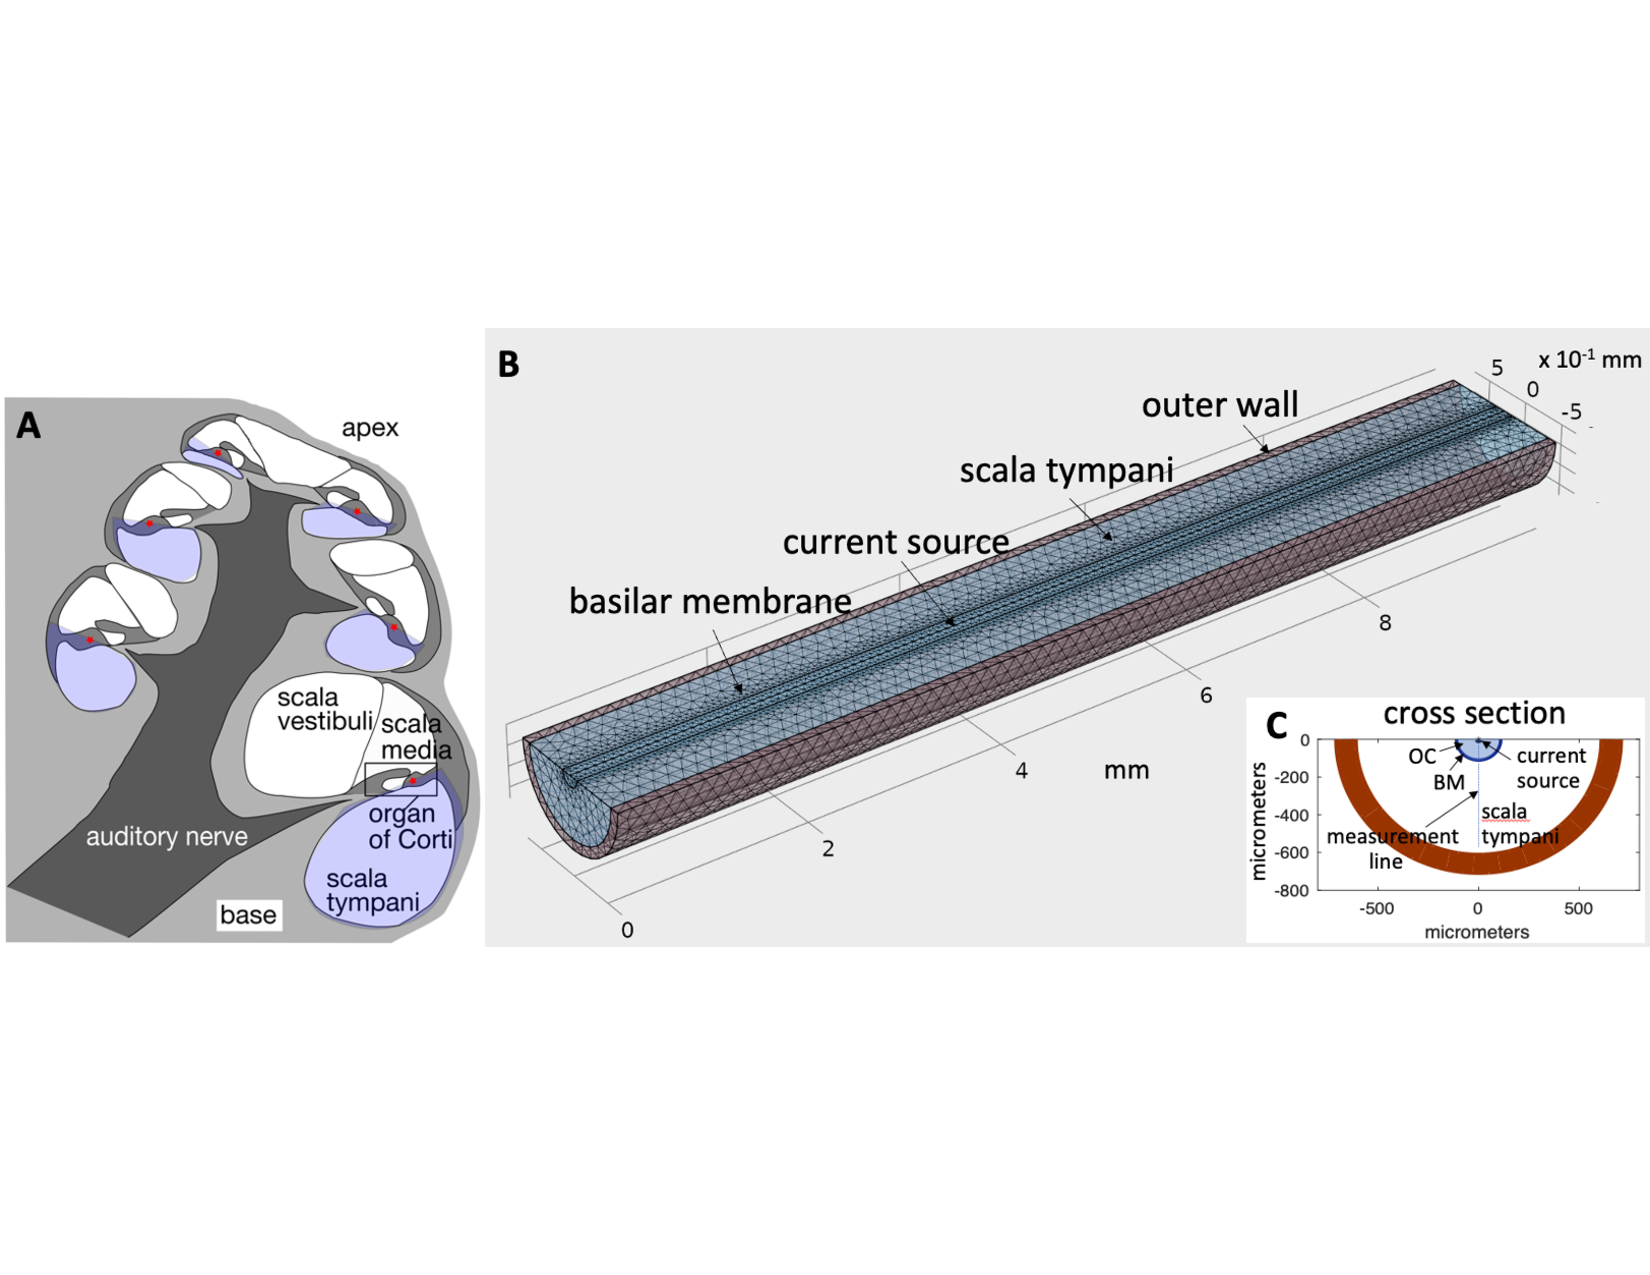
\includegraphics[width=\textwidth]{final_figures/modelfig.pdf}
\caption{\textbf{A} -- Cross-section of the gerbil cochlea, with the spiraling ST marked in blue. The red star represents the spiraling current source.  \textbf{B} -- Geometry of the model as it appears in the COMSOL Multiphysics user interface, representing an uncoiled version of the blue region in \textbf{A}. The outer wall is distinct from the larger fluid space, and the approximate position of the BM is marked by a half-cylindrical surface. The line current source can be seen on the flat surface.  \textbf{C} shows a cross-section 2.5 mm from the base, and the vertical line from source to wall is where simulated voltages are recorded. OC = organ of Corti, BM = basilar membrane.}
\label{geometry}
\end{figure}

\begin{figure}[h]
\centering
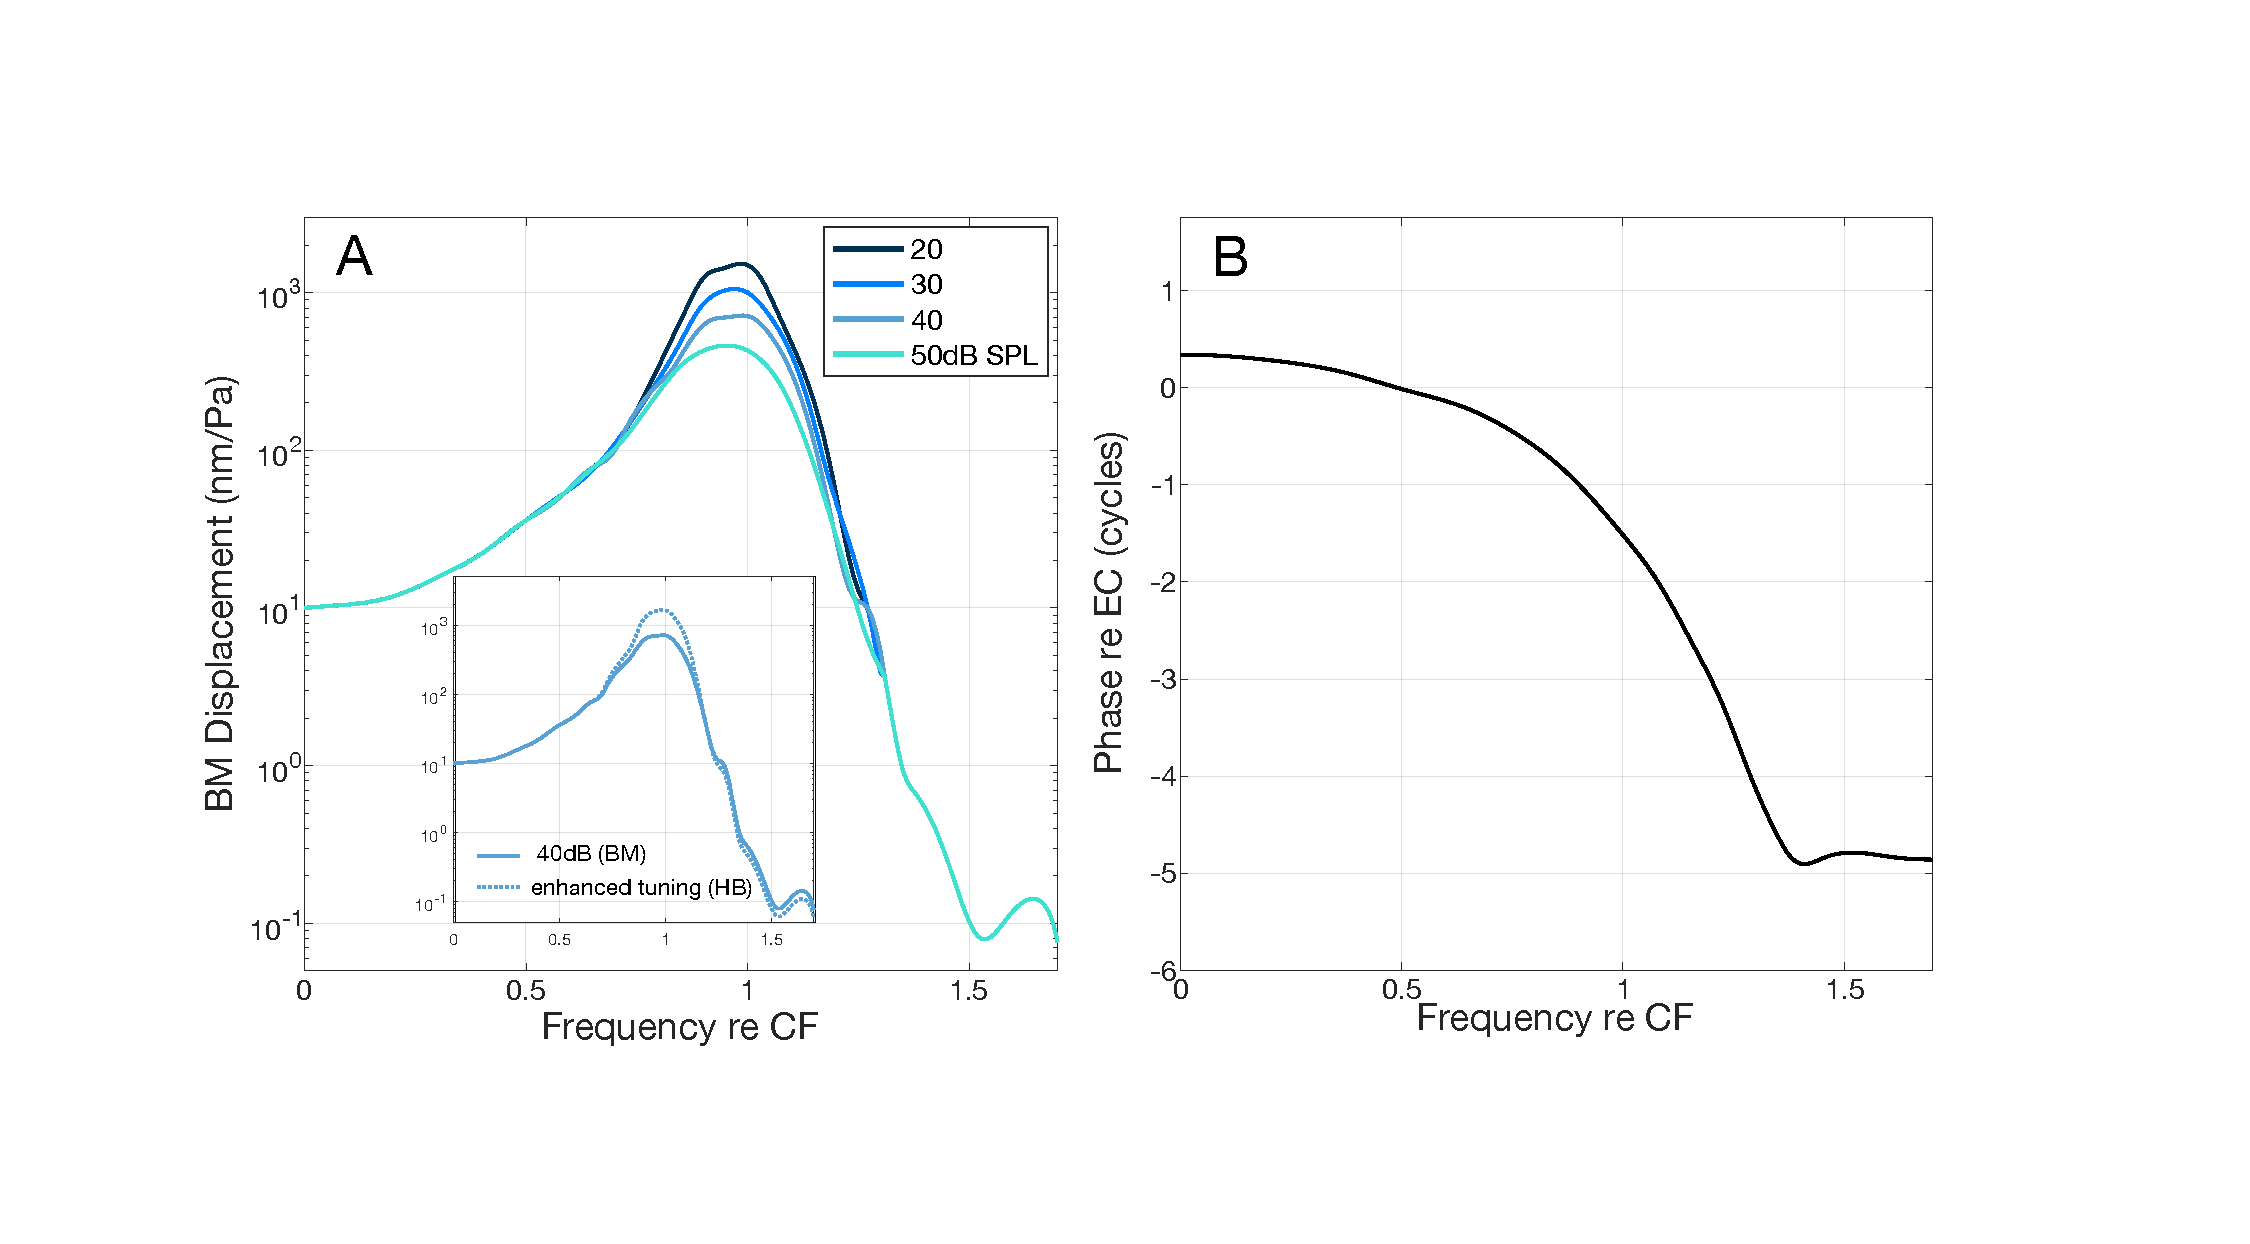
\includegraphics[width = \textwidth]{final_figures/input2.pdf}
\caption{Current source is initially assumed to be proportional to BM displacement shown here.  \textbf{A} Amplitude and \textbf{B} phase of BM displacement, based on gerbil data with CF 15.5 kHz \cite{RenPlos2011}, at sound pressure levels 20-50 dB SPL. The phase was nearly independent of SPL and the small variations were not included. Phase is shown referenced to the ear canal pressure. The data are plotted versus frequency/CF.  Inset in \textbf{A} shows enhanced tuning (of hair bundle = HB over basilar membrane) that will be applied to the 40 dB SPL input in one section of the results.}
\label{input1}
\end{figure}

\begin{figure}[h]
\centering
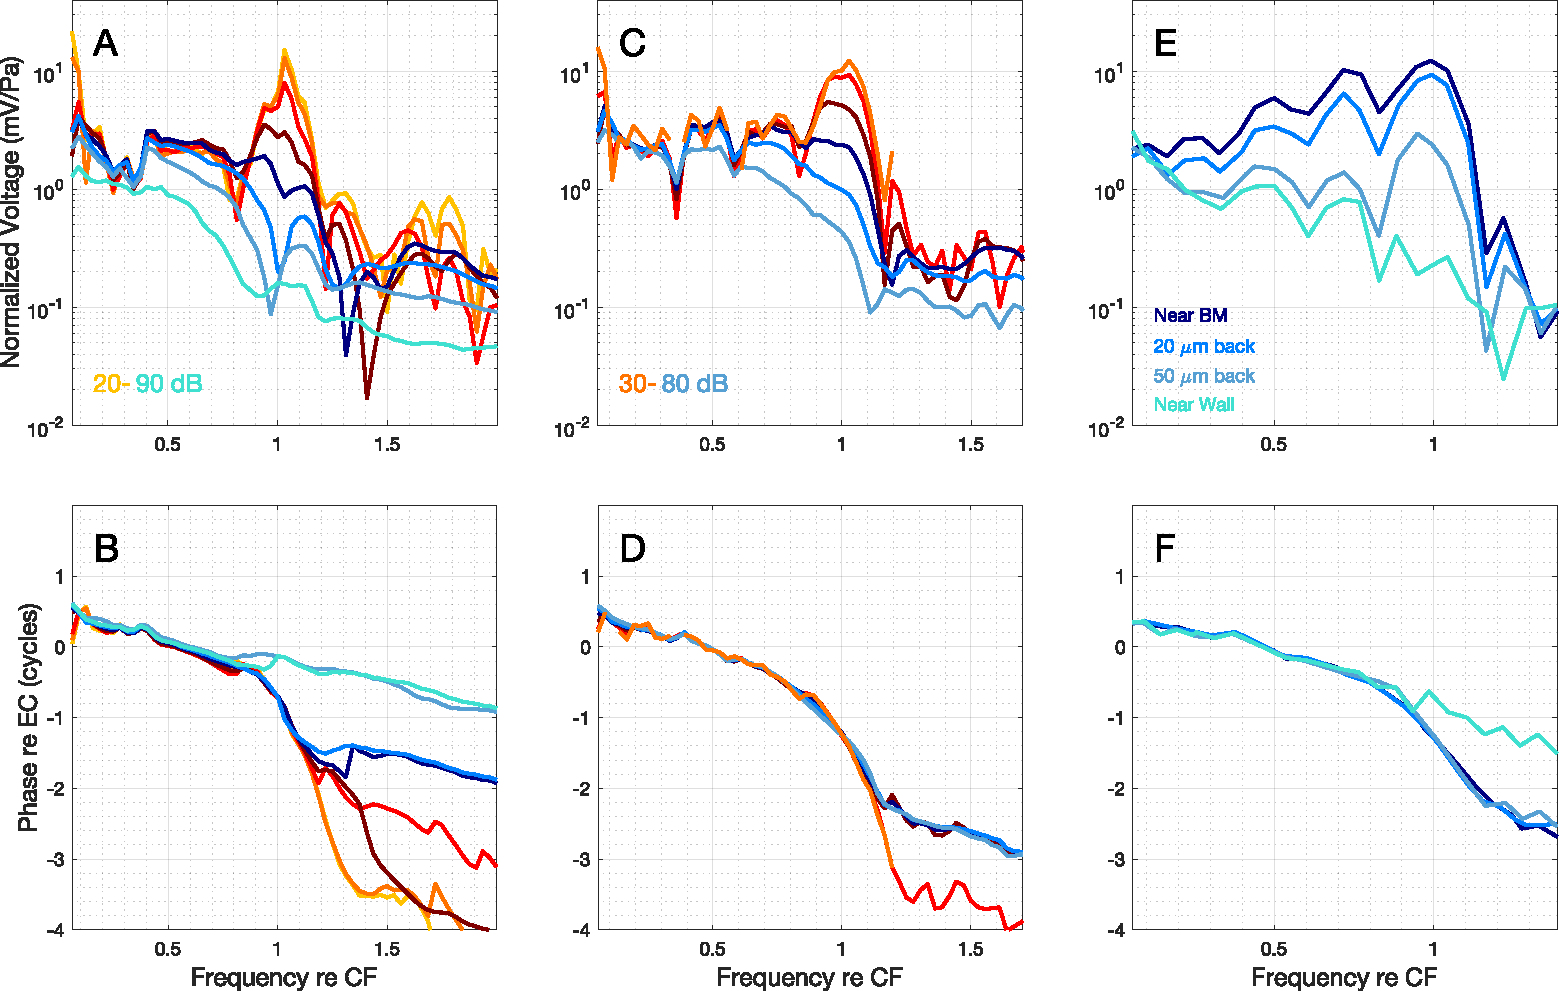
\includegraphics[width = \textwidth]{final_figures/data2.pdf}
\caption{Cochlear microphonic from experimental datasets. \textbf{A} and \textbf{B} -- Set 1, gerbil 712 \cite{fallah} amplitude and phase of CM measured close to ($\sim$ 20 $\mu$m from) the BM  at the 16 kHz CF location. SPL 20-90 dB in 10 dB intervals; \textbf{C} and \textbf{D} -- Set 2, gerbil 693 \cite{nankaliwang}  amplitude and phase of CM measured close to ($\sim$ 20 $\mu$m from) the BM at the 18 kHz CF location. SPL 30-80 dB in 10 dB intervals; \textbf{E} and \textbf{F} -- gerbil 693, amplitude and phase of CM at various distances from the BM in scala tympani at the 18 kHz CF location, 45 dB SPL.}
\label{data}
\end{figure}

\begin{figure}[h]
\centering
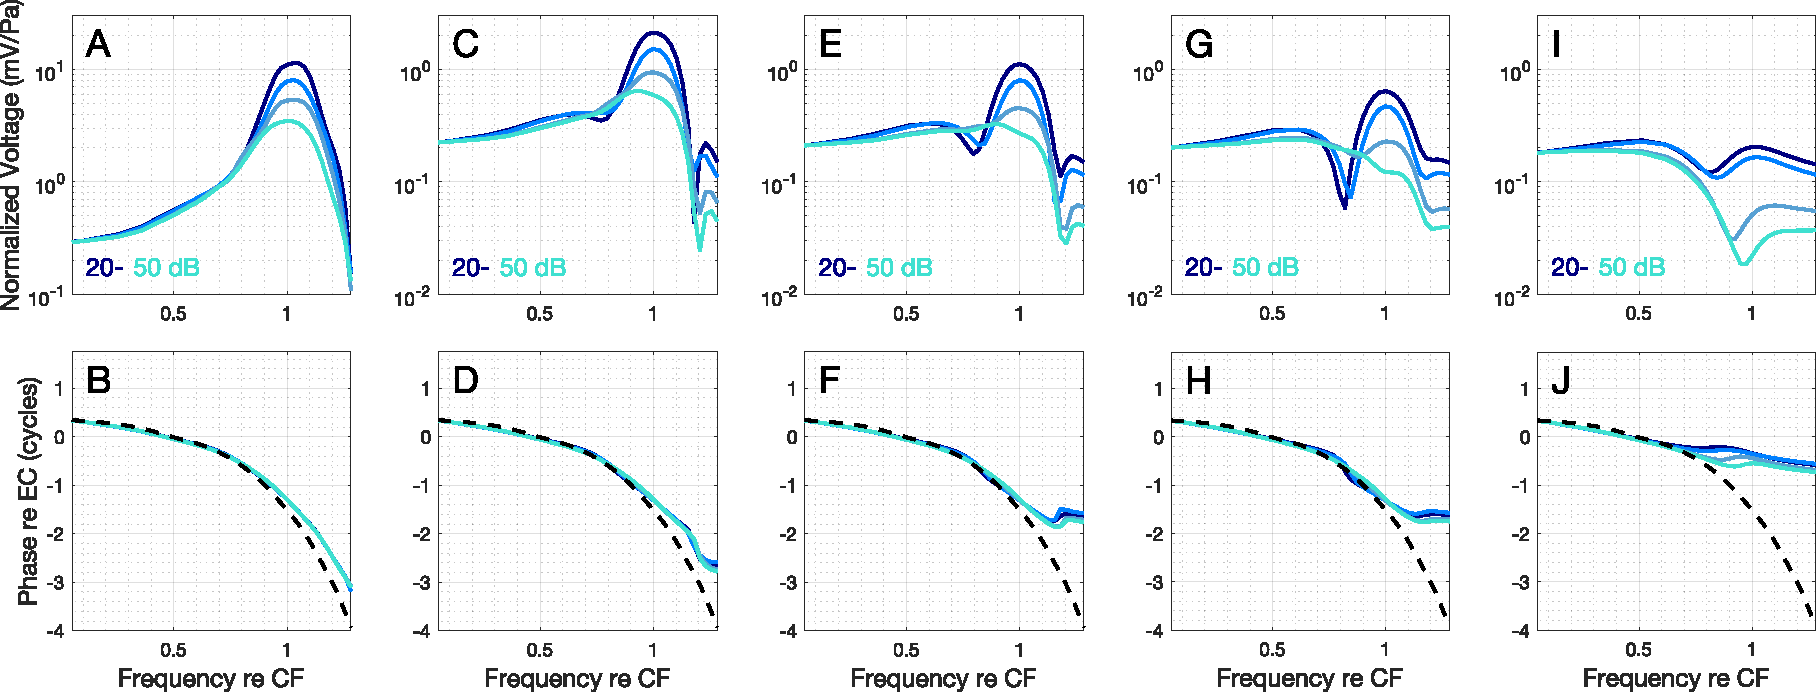
\includegraphics[width = \textwidth]{final_figures/distance.pdf}
\caption{CM prediction under the assumption that current is proportional to BM displacement. $K=50$, channel sensitivity = 33 pA/nm (starting value). Predictions are shown at five locations along the line segment 2.5 mm from the base of the cochlea (see Fig. \ref{geometry} \textbf{C}). Magnitude and phase: \textbf{A} and \textbf{B} -- at the position of the line current source; \textbf{C} and \textbf{D} -- 55 $\mu$m from the source; \textbf{E} and \textbf{F} -- 110 $\mu$m from the source; \textbf{G} and \textbf{H} -- 160 $\mu$m from the source; \textbf{I} and \textbf{J} -- 410 $\mu$m from the source. The dashed lines in the lower panels are the phase of the input (BM displacement) used to generate the current stimulus.}
\label{distance}
\end{figure}

\begin{figure}[h]
\centering
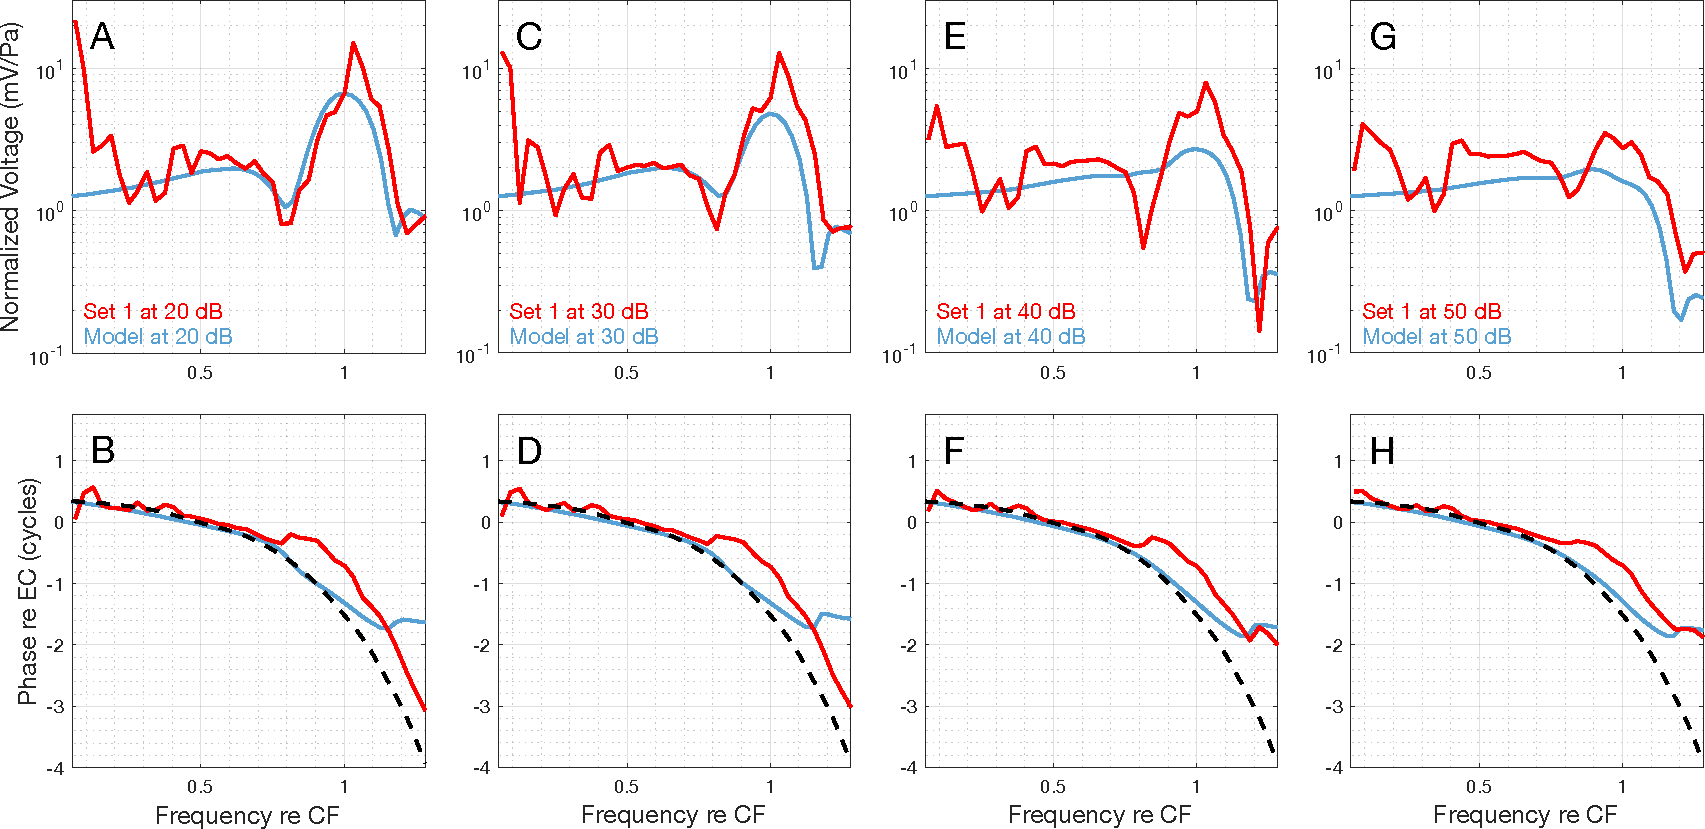
\includegraphics[width = \textwidth]{final_figures/compset110um.pdf}
\caption{Model LCM predictions 110 $\mu$m from the line current source ($\sim$ 20 $\mu$m from the BM) compared to experimental Set 1. Results (magnitude and phase) are shown at 20 (\textbf{A} and \textbf{B}), 30 (\textbf{C} and \textbf{D}), 40(\textbf{E} and \textbf{F}) and 50 dB SPL (\textbf{G} and \textbf{H}). CM predictions are based on the assumption that current is proportional to BM motion.  $K=50$, channel sensitivity is adjusted from starting value of 33 pA/nm to 200 pA/nm to align with the experimental result. The phase of the current stimulus is shown as a dashed line in the lower panels.}
\label{s1}
\end{figure}

\begin{figure}[h]
\centering
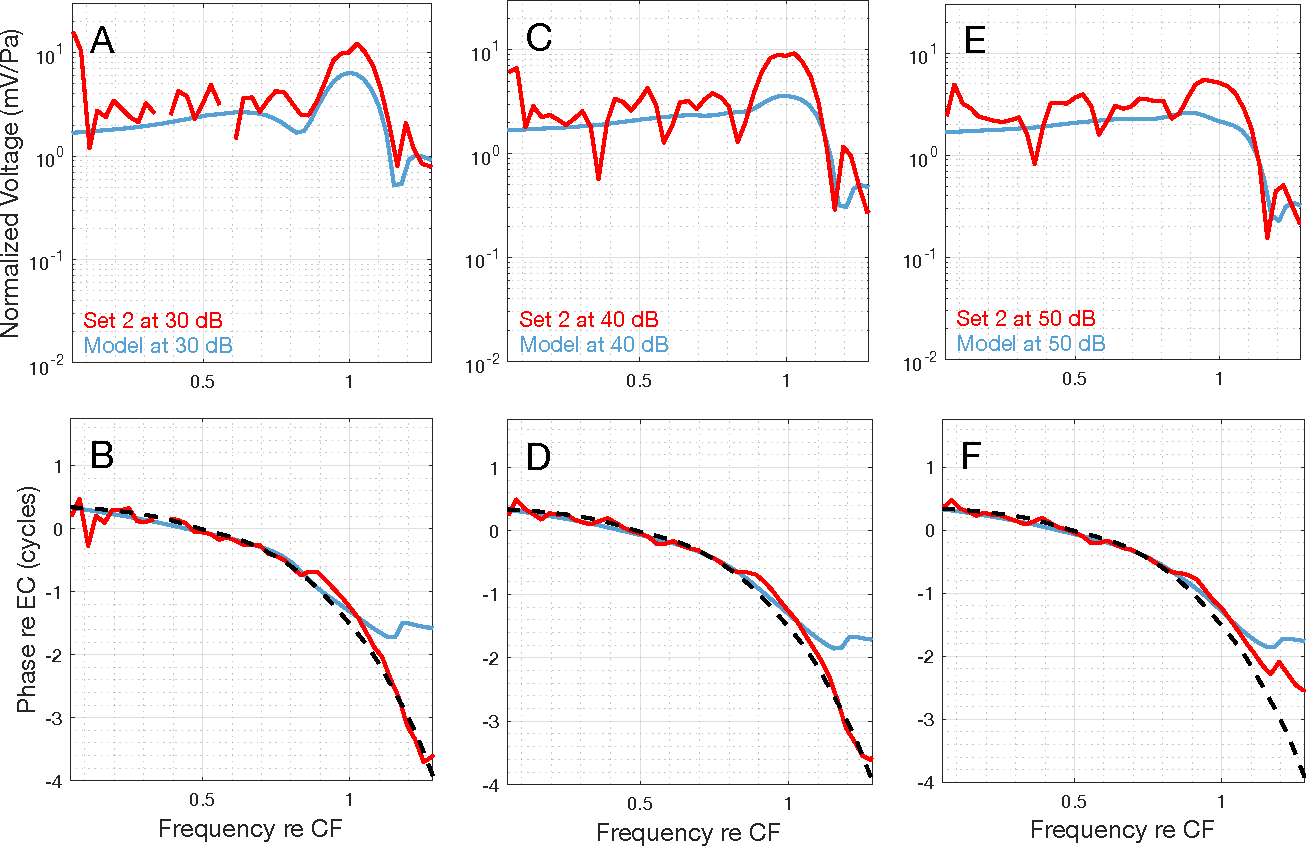
\includegraphics[width = \textwidth]{final_figures/compset2110um.pdf}
\caption{Model LCM predictions 110 $\mu$m from the line current source ($\sim$ 20 $\mu$m from the BM) compared to experimental Set 2. Results (magnitude and phase) are shown at 30 (\textbf{A} and \textbf{B}), 40 (\textbf{C} and \textbf{d}) and 50 dB SPL (\textbf{E} and \textbf{F}). CM predictions are based on the assumption that current is proportional to BM motion.  $K=50$, channel sensitivity is adjusted from starting value of 33 pA/nm to 260 pA/nm to align with the experimental result. The phase of the current stimulus is shown as a dashed line in the lower panels.}
\label{s2}
\end{figure}

\begin{figure}[h]
\centering
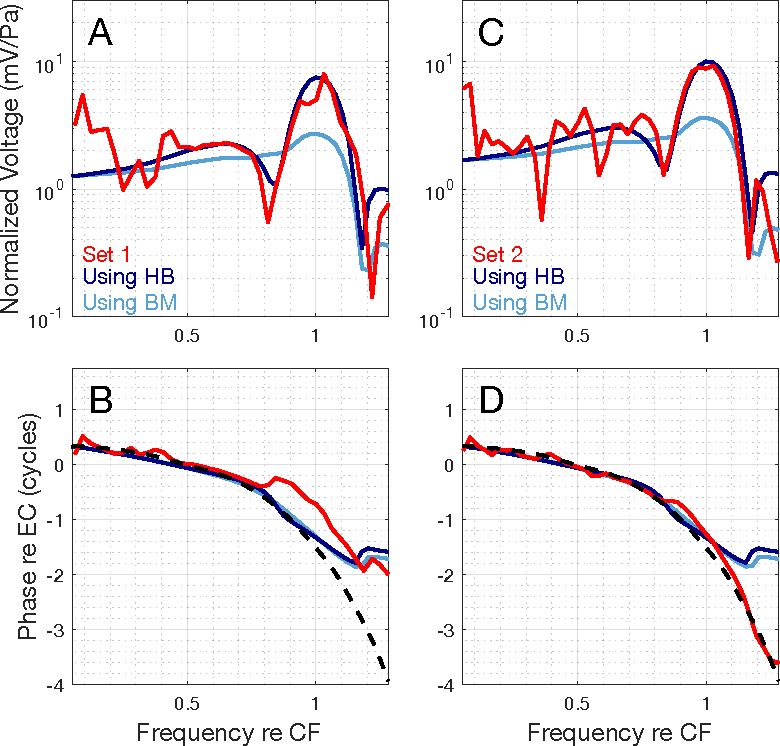
\includegraphics[width = 10 cm]{final_figures/comp hb110um.pdf}
\caption{Model LCM predictions 110 $\mu$m from the line current source compared to experimental data. Current source is based on the enhanced tuning of HB motion. Comparisons are made at 40 dB SPL. \textbf{A} and \textbf{B} -- Set 1 comparison. $K=50$ and channel sensitivity adjusted from starting value to to 200 pA/nm (same as Fig. \ref{s1}). \textbf{C} and \textbf{D} -- Set 2 comparison, $K=50$ and channel sensitivity adjusted to 260 pA/nm (same as Fig. \ref{s2}).  The phase of the current stimulus is shown as a dashed line in each phase plot.  }
\label{sTF}
\end{figure}

\begin{figure}[h]
\centering
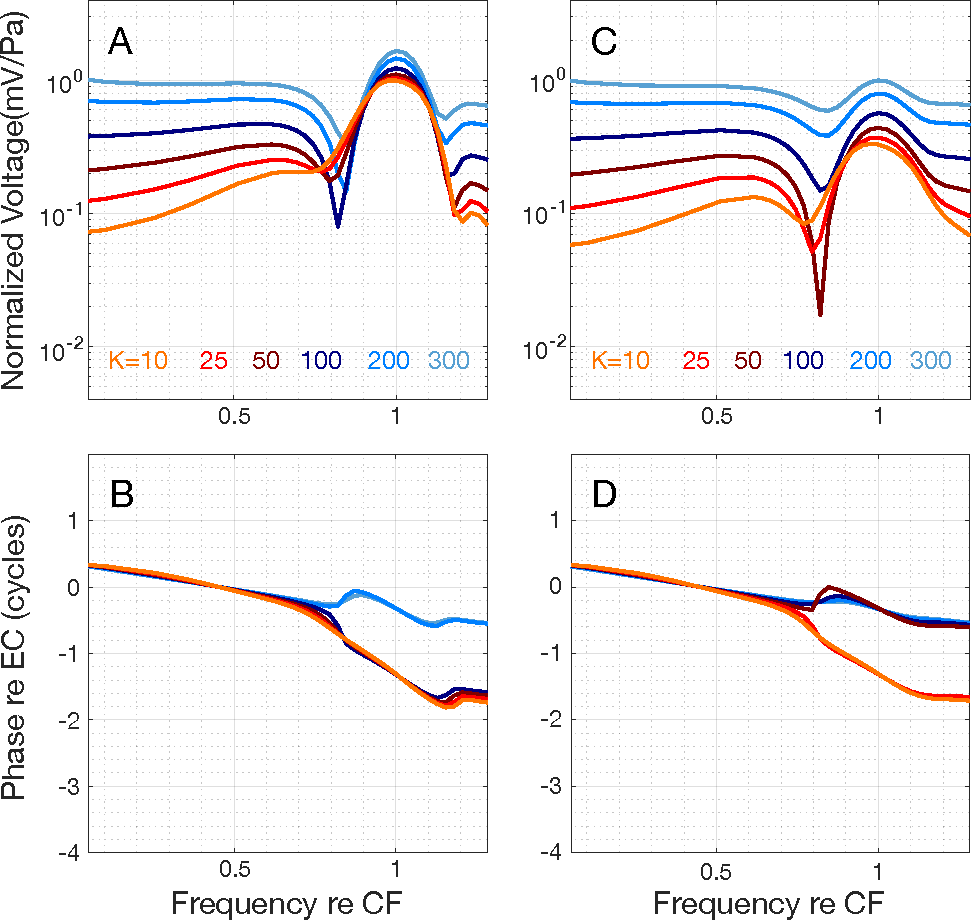
\includegraphics[width = 10 cm]{final_figures/k.pdf}
\caption{Effect of variations in lateral wall conductivity, $\sigma_W = \sigma/K$, where $\sigma$ is the conductivity of the ST saline solution.  Predicted CM at 20 dB SPL with $K$=10, 25, 50, 100, 150 and 300. \textbf{A} and \textbf{B} -- 110 $\mu$m from the line current source; \textbf{C} and \textbf{D} -- 210 $\mu$m from the line current source. Channel sensitivity is set to 33 pA/nm.}
\label{K}
\end{figure}

\begin{figure}[h]
\centering
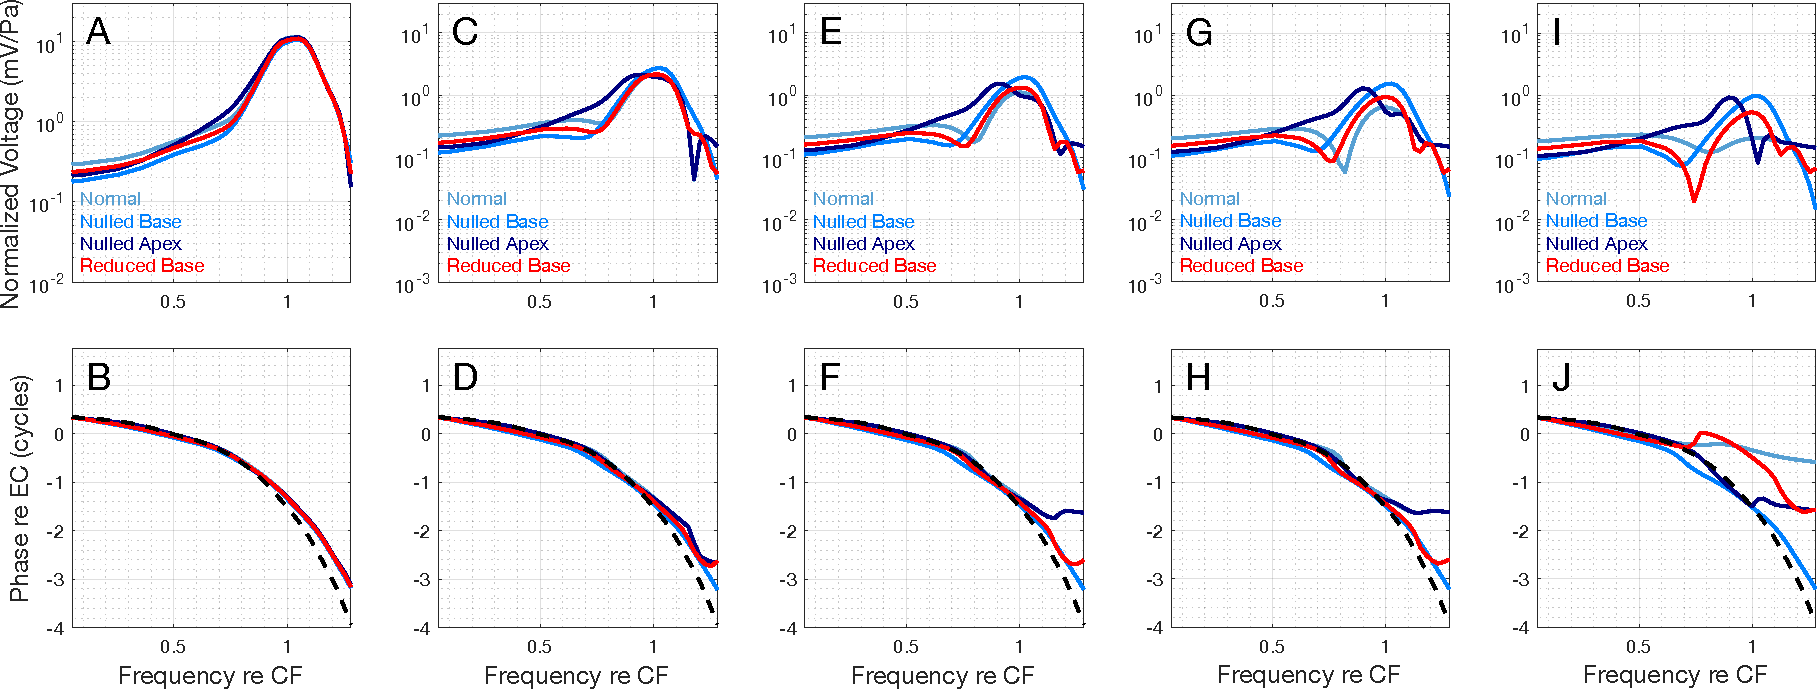
\includegraphics[width = \textwidth]{final_figures/Modified Damage Figure.pdf}
\caption{Effect of nulling or reducing the current source basal or apical of the measurement location (19.5 kHz CF place). Panel sets show magnitude and phase at various distances from the current source . The original current source, based on BM displacement tuning, and the original channel sensitivity, 33 pA/nm, are used. In the nulled-base case, the current source from the base to the 21 kHz place is set to 0. In the reduced-base case the current source from the base to the 21 kHz place is reduced by half. In the nulled-apex case, current from the apex to the 18 kHz place is set to 0. SPL = 20 dB SPL, $K=50$. \textbf{A} and \textbf{B} -- CM predictions at the position of the line-current source; \textbf{C} and \textbf{D} -- 55 $\mu$m from the line current source; \textbf{E} and \textbf{F} -- 110 $\mu$m from the line current source; \textbf{G} and \textbf{H} -- 160 $\mu$m from the line current source; \textbf{I} and \textbf{J} -- 410$\mu$m from the line current source.  The phase of the current stimulus is shown as a dashed line in the lower panels.}
\label{damage}
\end{figure}

\begin{figure}[h]
\centering
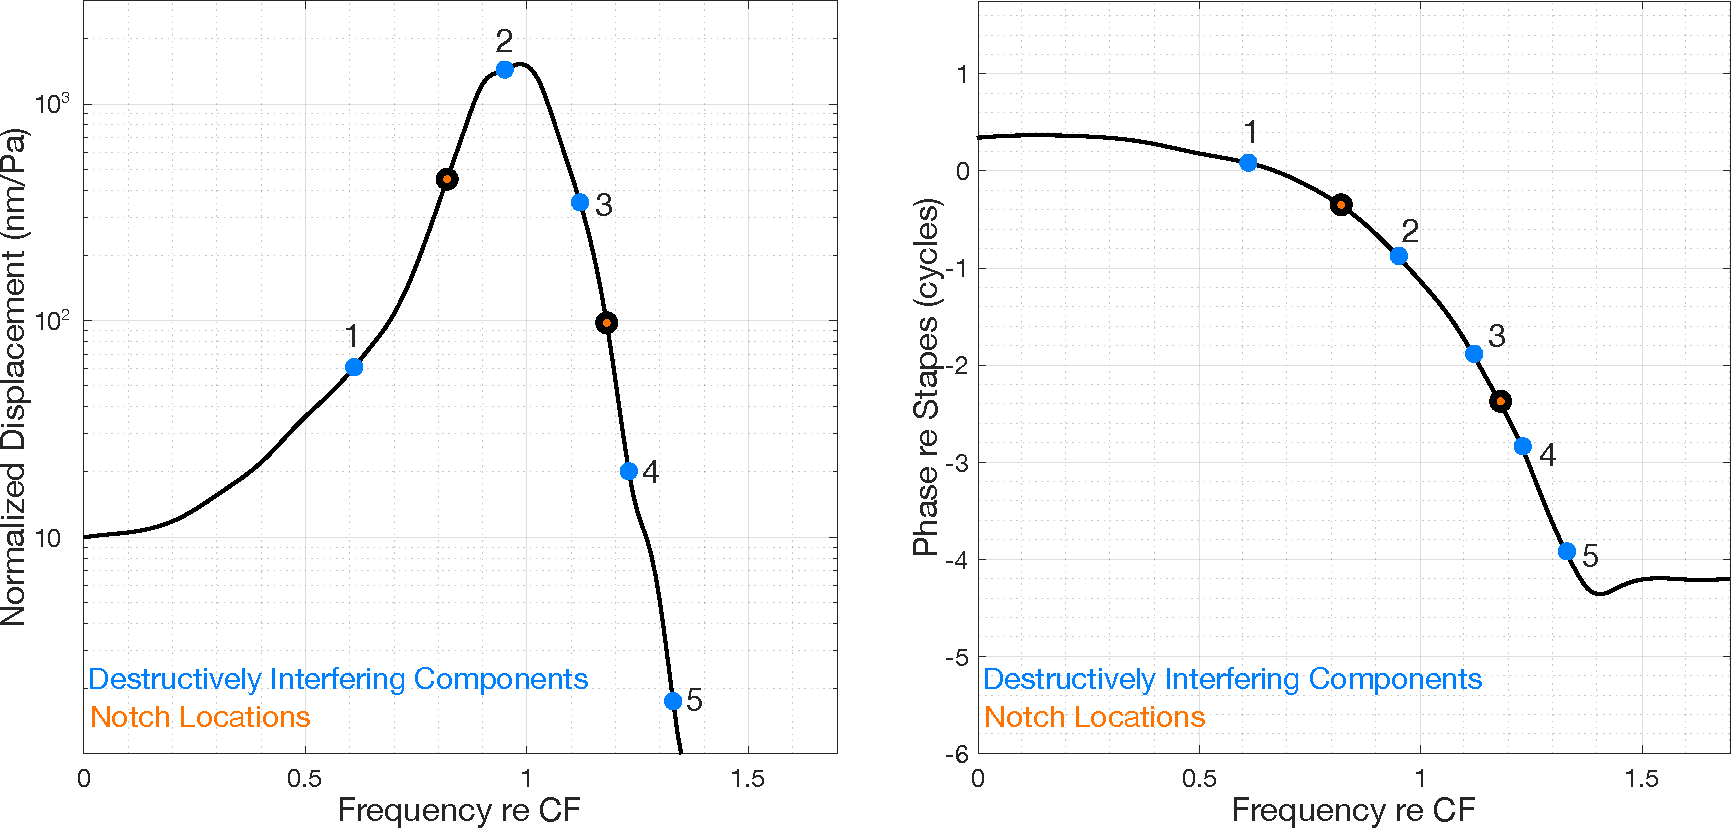
\includegraphics[width =  \textwidth]{final_figures/NotchExp2.pdf}
\caption{Exploration of the basis of prominent notches. Amplitude and phase of the basilar membrane displacement data used to generate the model input. As in Fig. \ref{input1}, except here the reference is stapes (so that all phase variation occurs within the cochlea). Highlighted in orange are the values of the amplitude and phase at the frequencies where notches appear in our model predictions, $\sim$ 0.8CF and 1.2CF. These correspond to phases of 0.36 and 2.36 cycles. Highlighted in blue are values corresponding to frequencies where the phases are half of a cycle off from the phase at the notch frequencies. Current components at the frequencies in blue will interfere destructively with those in orange.}
\label{notchcancel}
\end{figure}

{\begin{figure}[h]
\centering
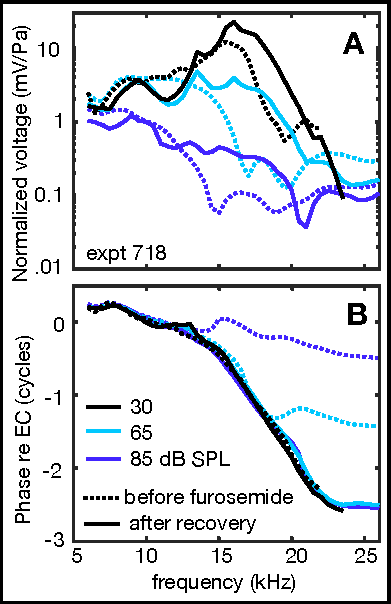
\includegraphics[width=6 cm]{final_figures/Wang2.pdf}
\caption{Experimental data related to model prediction with basal current nulled or reduced. CM measured close to the BM, before administering furosemide and after recovery from furosemide (3.5 hrs later). \textbf{A} Normalized voltage amplitude. \textbf{B} Phase relative to ear canal.  Note that traveling wave phase accumulation is present even at high SPLs after recovery, indicating that the response was more local after recovering from furosemide than it was before furosemide. A reasonable explanation is that the more basal region had not recovered fully from furosemide, and was partially nulled, reducing the interference of non-local basal current.}
\label{Wang}
\end{figure}}

\begin{figure}[h]
\centering
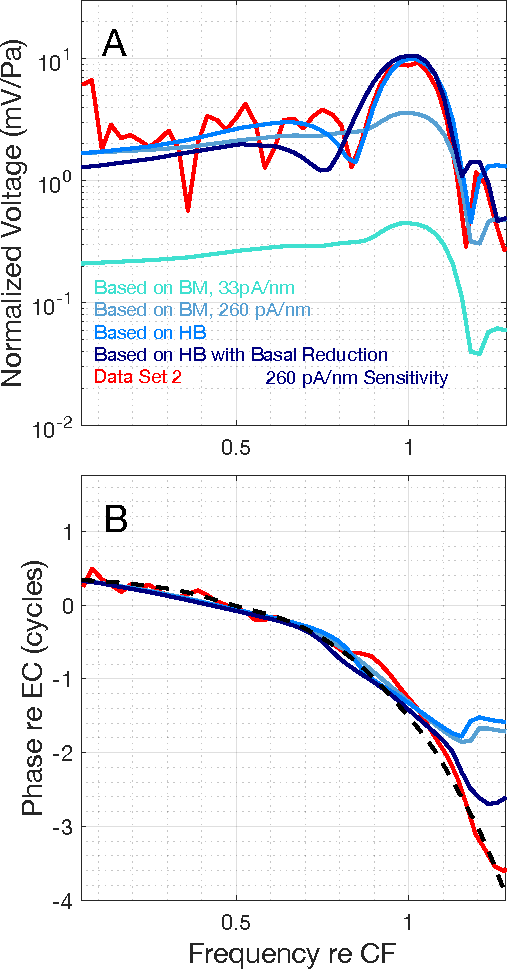
\includegraphics[width = 6cm]{final_figures/finalcom_yi.pdf}
\caption{Experimental data Set 2 (40 dB SPL) and LCM predictions as the current source representation progressed.  The current source was initially represented in the model as proportional to BM displacement and transducer gain estimated from \textit{in vitro} findings (cyan), then with increased transducer sensitivity (light blue), then enhanced tuning (medium blue) and finally reduction of the current sources basal to the measurement location (dark blue), which produced a more realistic phase accumulation. The phase of the current source was not changed and is included in a dashed line.}
\label{finalcomparisonYi}
\end{figure}

\clearpage

\bibliography{mybib}

\end{document}
